\documentclass[12pt]{report}

\usepackage[a4paper,width=150mm,top=25mm,bottom=25mm,bindingoffset=6mm]{geometry}
\usepackage[onehalfspacing]{setspace}
\usepackage{ucs}
\usepackage[table,xcdraw]{xcolor}
\definecolor{mColor1}{rgb}{0.9,0.9,0.9}

\usepackage{fancyhdr}
\pagestyle{fancy}
\fancyhead{}
\renewcommand{\chaptermark}[1]{\markboth{#1}{}}
\renewcommand\sectionmark[1]{\markright{\thesection\ #1}}

\fancyhead[LO, RE]{\leftmark}
\fancyhead[LE, RO]{\rightmark}

\usepackage{titlesec, blindtext, color}
\definecolor{gray75}{gray}{0.75}
\usepackage{mathptmx}
\usepackage[utf8]{inputenc}
\usepackage[T1]{fontenc}
\usepackage[ngerman]{babel}

\usepackage{amsmath,amssymb,amstext,amsthm,mathtools}
\usepackage{url}
\usepackage{caption}
%\usepackage[belowskip=-5pt,aboveskip=0pt]{caption}
\usepackage{subcaption}

\usepackage{float}
\usepackage{lscape}
\usepackage{pdfpages}
\usepackage{rotating}
\usepackage{graphicx}
\setlength\parindent{0pt}
\usepackage{hyperref}
\usepackage{acronym}
\usepackage{textcmds}
\usepackage{longtable}
\usepackage[export]{adjustbox}
\usepackage{upgreek}
\usepackage{dsfont}
\usepackage{tensor}
\usepackage{amsbsy}


\DeclareMathAlphabet{\mathcal}{OMS}{cmsy}{m}{n}
\SetMathAlphabet{\mathcal}{bold}{OMS}{cmsy}{b}{n}

\usepackage{listings, lstautogobble}
\usepackage{textcomp}
\definecolor{yo}{rgb}{0.9,0.6,0}
\definecolor{Gray}{gray}{0.9}
\definecolor{listinggray}{gray}{0.9}
\definecolor{lbcolor}{rgb}{0.95,0.95,0.95}
\lstset{
	backgroundcolor=\color{lbcolor},
	tabsize=4,
	rulecolor=,
	language=python,
        basicstyle=\scriptsize,
        upquote=true,
        aboveskip={1.5\baselineskip},
        columns=fixed,
        showstringspaces=false,
        extendedchars=true,
        breaklines=true,
        prebreak = \raisebox{0ex}[0ex][0ex]{\ensuremath{\hookleftarrow}},
        frame=lines,
        showtabs=false,
        showspaces=false,
        showstringspaces=false,
        identifierstyle=\ttfamily,
        keywordstyle=\color[rgb]{0.55,0,0},
        alsoletter={/,*,[,]},%
        otherkeywords={},
        morekeywords=[2]{with, as},
        morekeywords=[3]{},
        emph={self},          % Custom highlighting
		emphstyle=\color[rgb]{0.1,0.3,1},
		emph={[2]f},          % Custom highlighting
		emphstyle={[2]\color[rgb]{0.1,0.5,0.1}},
		emph={[3]__init__},          % Custom highlighting
		emphstyle={[3]\color[rgb]{0.1,0.3,1}},
		emph={[4]open,str,print,KeyError},          % Custom highlighting
		emphstyle={[4]\color[rgb]{0.2,0.6,0.8}},
        commentstyle=\color[rgb]{0.3,0.3,0.3},
        stringstyle=\color[rgb]{0.133,0.545,0.133},
        	autogobble=true
}
\lstnewenvironment{ttlisting}{\lstset{basicstyle=\scriptsize}}{}

\usepackage{color}
\usepackage[section]{placeins}

\newenvironment{simplechar}{%
	\catcode`\$=12
	\catcode`\&=12
	\catcode`\#=12
	\catcode`\^=12
	\catcode`\_=12
	\catcode`\~=12
	\catcode`\%=12
	\catcode`\"=12
	\catcode`\'=12
	}{}{}

\newtheoremstyle{dotless}{}{}{\itshape}{}{\bfseries}{}{ }{}

\theoremstyle{dotless}

\newtheorem{thm}{Theorem}
\newtheorem{defn}[thm]{Definition} 
\newtheorem{exmp}[thm]{Example}
\theoremstyle{definition}


\begin{document}

\begin{titlepage}
	Warum bin ich nicht einfach Staubsaugervertreter geworden? 
\end{titlepage}

\tableofcontents

\chapter{Allgemeiner Unsinn für Grundlagen aktuarieller Kalkulation}

\subsubsection{Sparten}
\begin{itemize}
	\item Umfasst Leben, Kranken, Komposit, Pensionen
	\item Leben, Kranken, Pensionen sind zusammen Personenversicherung
	\item Komposit: Schaden/Unfall
	\item Besonders: priv. Unfall ist Komposit
\end{itemize}

\begin{defn} (Farny)
	Deckung eines im Einzelnen ungewissen, insgesamt schätzbaren Mittelbedarfs unter Nutzung von Ausgleichsmechanismen im Kollektiv.
\end{defn}

\subsubsection{Wichtigste Zweige Komposit}
\begin{itemize}
	\item Sachversicherung
	\item Haftpflichtversicherung
	\item Transportversicherung
	\item Technische Versicherung
\end{itemize}

\subsubsection{Prämienzahlweise}
\begin{itemize}
	\item üblicherweise jährlich
	\item bei unterjährigen Zahlung Ableitung aus Jahresprämie
\end{itemize}

\subsubsection{Diskont und Barwert}
\begin{itemize}
	\item Diskontfunktion bei einjährigem Zinssatz $r$: $D(t)=(1+r)^{-t}$
	\item Diskontfunktion bei Rechnungszins $i$: $D(t) = (\frac{1}{1+i})^t \eqqcolon v^t$
	\item Barwert aller Leistungen: $L=\sum_{t=0}^{\bar{n}}D(t)\cdot L_t$
	\item Barwert aller Prämien: $P=\sum_{t=0}^{\bar{n}}D(t)\cdot P_t$
	\item Barwert aller Kosten: $K=\sum_{t=0}^{\bar{n}}D(t)\cdot K_t$
	\item Sicherheitszuschlag: Eintrittswahrscheinlichkeit erhöhen, Diskont verringern
\end{itemize}

\subsubsection{Äquivalenzprinzip}
\begin{align}
	\text{(ÄP I):} \ \ \ \ \ \ \ \ \ \ \ \ \ \ \ E(P)=E(L) \\
	\text{(ÄP II):} \ \ E(P)=E(L)+E(K)
\end{align} 

\begin{defn} \ \\
	\begin{itemize}
		\item Falls $L$ und $P$ das Äquivalenzprinzip erfüllen, dann hei{\ss}t $P_{\bullet}$ Nettorisikoprämienprozess und $P_t$ Nettorisikoprämie.
		\item $L$ und $P$ erfüllen ÄP und $\exists \ w_t$ Wahrscheinlichkeit der Prämienzahlung $P_t$ und $\bar{P}$ konstant mit $E(P_t)=\bar{P}\cdot w_t \ \forall \ t \in \{0,...,\bar{n}\}$. $\bar{P}$ konstante Nettorisikoprämie.
		\item Bruttorisikoprämie: $P^+ \coloneqq \bar{P}+c$ mit $c>0$ Sicherheitszuschlag.
		\item Alternativ: Sicherheitszuschlag bereits in Nettorisikoprämie enthalten
	\end{itemize}
\end{defn}

\subsubsection{Notation}
\begin{itemize}
	\item $\bar{n}$: Modelldauer
	\item $t$: Zeit in jahren
	\item $r$: einjähriger konstanter Zinssatz
	\item $D(t)$: Diskontfunktion
	\item $L_t$: Versicherungsleistung in $t$
	\item $q_t$: Eintrittswahrscheinlichkeit Leistungsfall in $t$
	\item $P_t$: Prämienzahlung in t
	\item $w_t$: Wahrscheinlichkeit Prämienzahöung in $t$
	\item $K_t$: Kosten in $t$
	\item $L$: Leistungsbarwert
	\item $P$: Prämienbarwert
	\item $K$: Kostenbarwert
\end{itemize}

\subsubsection{Sterbetabeln}

\begin{figure}[ht]
	\centering
	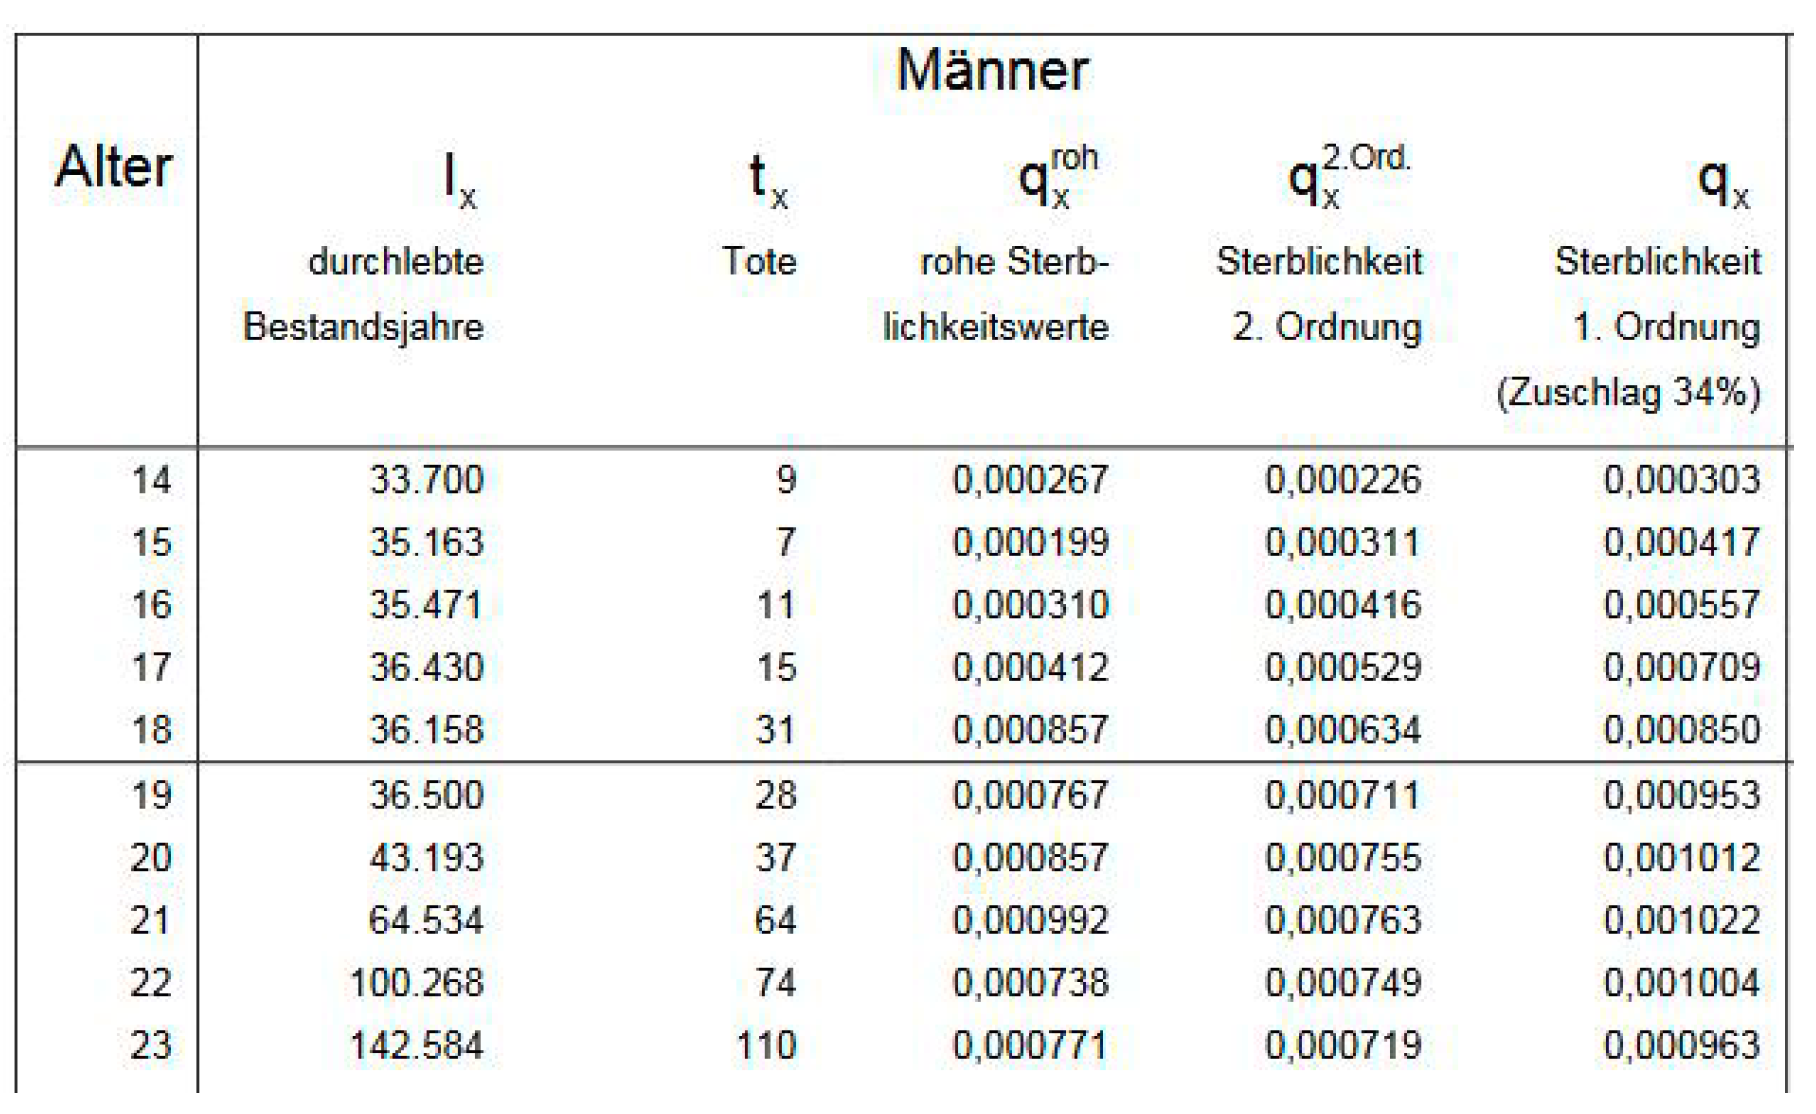
\includegraphics[width = .8\textwidth]{Bilder/Sterbetafelbsp.png}
\end{figure}

\subsubsection{Allgemeine aktuarielle Herangehensweise, spartenübergreifend ähnliches Standardvorgehen zur Bewertung zufälliger zukünftiger Versicherungsleistungen}
\begin{itemize}
	\item Beobachtung von Vergangenheit (Daten) zur Vorhersage der Zukunft
	\item Anpassung geeigneter Wahrscheinlichkeitsverteilung
	\item Sorgfalt bzgl. möglicher Änderungen von Annahmen im zeitlichen Verlauf
	\item typischerweise konstante Prämienhöhe
	\item Risiko steigt mit zeitlichem Verlauf
	\item Ansparprozess und Entsparprozess
\end{itemize}

\subsubsection{Rückstellungen}
\begin{itemize}
	\item Ziel: Sicherstellung der dauernden Erfüllbarkeit
	\item versicherungstechnische Rückstellungen wichtigste Passivposition in der Bilanz des VU
	\item hohe bedeutung für interne Unternehmensbewertung
	\item Einfluss auf Besteuerung des VU
	\item Unterschied zwischen bilanzieller und einzelvertraglicher versicherungsmathematischer Deckungsrückstellung
	\item Deckungskapitel $\hat{=}$ Erwarteter Barwert künftiger Leistungen - Erwarteter Barwert künftiger Beiträge
\end{itemize}

\subsubsection{Rückstellungen in der Schadenversicherung}
\begin{itemize}
	\item Einzelschadenreserven: für noch nicht vollständig abgewickelte Schäden
	\item Deckungsrückstellungen: für Haftpflicht, Unfallrenten und Beitragsrückgewähr in Unfall
	\item Spätschadenpauschalreserve: für IBNR
	\item Schwankungsrückstellung: relevant für Zweige mit stark variierenden Schadenfällen 
\end{itemize}

\subsubsection{Prämienprinzipien}
\begin{itemize}
	\item Ziel: Zuordnung angemessener Prämie durch Bemessung geeigneter Sicherheitszuschläge
	\item Deckung der Leistungsfälle und zusätzliche Prämie zur Bereitschaft der Risikoübernahme durch VU (Sicherheitszuschlag SZ(X))
	\item Prämienprinzipien $H(X) \coloneqq E(X)+SZ(X)=P^+$, $X$ ist das versicherte Risiko
	\item Sicherheitszuschlag bei gleichem EW höher, wenn Risiko gefährlicher
	\item Nettorisikoprinzip: $H(X)=E(X)$
	\item Erwartungswertprinzip: $H(X)=E(X)+\delta \cdot E(X) = (1+\delta) \cdot E(X)$
	\item Varianzprinzip: $H(X)=E(X) + \delta \cdot Var(X)$
	\item Standardabweichungsprinzip: $H(X)=E(X) + \delta \cdot \sqrt{Var(X)} = E(X) + \delta \cdot \sigma(X)$ (anders als andere nicht additiv)
	\item Exponentialprinzip: $H(X) = \frac{1}{a} \cdot ln(M_X(a)) = \frac{1}{a}\cdot ln(E[e^{aX}])$ mit $a>0$, Monumenterzeugender Funktion $M_X$, entspricht näherungsweise Varianzprinzip mit $\delta = \frac{a}{2}$ und ist ein Spezialfall des Nutzenprinzips
	\item Es gilt: $\Gamma(1,\lambda) = Exp(\lambda)$ und $X_i \sim \Gamma(a_i,\lambda), \ i=1,...,n$ unabhängig \\ $\Rightarrow \sum_{i=1}^n X_i \sim \Gamma (\sum_{i=1}^n a_i, \lambda)$
\end{itemize}

\subsubsection{Nettorisikoprämie berechnen}
\begin{flalign}
	E(P) = \sum_{t=0}^n w_t \cdot D(t) \cdot P_t \\
	E(L) = \sum_{t=0}^n q_t \cdot D(t) \cdot L_t \\
	E(P)=E(L)
\end{flalign}
$w_t, q_t$ sind die Wahrscheinlichkeiten, einer positiven Prämien- bzw. Leistungszahlung.


\begin{defn}
	(Ungleichung von Cantelli)
	\begin{align}
		P(X>E(X)+c) \leq \frac{Var(X)}{c^2+Var(X)} \\
		\text{Hinweis: SZ wird hier stark überschätzt.} \\
		c \leq \sqrt{\frac{1 - \epsilon}{\epsilon}} \cdot \sqrt{Var(X)}
	\end{align}

\end{defn}

\subsubsection{Beispiele Risikoma{\ss}e}
\begin{itemize}
	\item Erwartungswert $E(X)$
	\item Varianz $Var(X)$
	\item Schiefe $\gamma(X)$ (Symmetriema{\ss}
	\item Tail-Whk $P(X>t)$
	\item Ruin- und Verlustwahrscheinlichkeiten
	\item Bernoulli-Nutzen
	\item Value at Risk (VaR), Expected Shortfall, Tail Value at Risk (TVaR)
\end{itemize}

\begin{defn}
\begin{align}
	\text{Additivität: } H(X+Y)=H(X)+H(Y) \ \forall \ X,Y \text{stochastisch unabhängig} \\
	\text{Subadditivität: } H(X+Y) \leq H(X)+H(Y) \ \forall \ X,Y \text{stochastisch unabhängig} \\
	\text{Erwartungswertübersteigend: } SZ(X) \geq 0
\end{align}
\end{defn}

% To-Do: Folie 112-114 beantworten und einfügen

\begin{defn}
	(1) Ein Kollektiv stellt eine Zusammenfassung von Risiken dar, die durch gleichartige Gefahren bedrohnt sind. Kollektiv bedeutet nicht zwangsläufig, dass es sich um \textit{versicherte Risiken} handelt. \\
	(2) Der Risikoausgleich im Kollektiv stellt neben dem Ausgleich in der Zeit ein wesentliches Funktionsprinzip von Versicherungen dar. \\
	(3) Ein Kollektiv hei{\ss}t homogen, falls alle Risiken des Kollektivs dieselbe Verteilung besitzen, anderenfalls hei{\ss}t es heterogen. \\
	(!) Hinweis: Homogenität und Unabhängigkeit sind keine notwendige Voraussetzung für Risikoausgleich im Kollektiv. Im Gegenteil: gleicht sich durch gegenläufige Abhängigkeiten z.T. aus.
\end{defn}

\subsubsection{Risikoausgleich}
\begin{itemize}
	\item Das Überschreiten einer prozentualen Maximalabweichung vom Erwartungswert wird bei wachsendem Kollektiv immer unwahrscheinlicher.
	\item Risikoausgleich im Kollektiv erfolgt insofern, als dass der Variationskoeffizient als versicherungsspezifisches Risikoma{\ss} für wachsende Bestände gegen 0 konvergiert.
	\item Mit zunehmender Zahl von Risiken sinkt die relative Abweichung des arithmetischen Mittels vom Erwartungswert.
\end{itemize}

\begin{defn}
$Y_i\geq$ kumulierter Gesamtaufwand des $i$-ten Risikos. $S^{ind}=\sum_{i=1}^nY_i $.
	\begin{align}
		\text{Durch Linearität des EWs: } E(S^{ind})=\sum_{i=1}^n E(Y_i) \\
		\text{Da } Y_i \text{ unabhängig: } Var(S^{ind})=\sum_{i=1}^n Var(Y_i) \\
		\text{Variationskoeffizient: } Vko(S^{ind})=\frac{\sqrt{\sum_{i=1}^nVar(Y_i)}}{\sum_{i=1}^nE(Y_i)}
	\end{align}
\end{defn}

\begin{defn}
	Erste und zweite Formel von Wald. N die Schadenzahl. \\
	(1) $E(S^{koll})=E(N)\cdot E(X)$ \\
	(2) $Var(S^{koll})=E(N) \cdot Var(X) + (E(X))^2 \cdot Var(N)$
\end{defn}

\subsubsection{Gegenüberstellung individuelles und kollektives Modell}
\begin{itemize}
	\item dieselbe Gesamtsumme $S^{ind}=S^{koll}$
	\item ind: $n =$ Anzahl individuell betrachteter Risiken (deterministisch), koll: $N =$ Anzahl der Finanzaufwände, Zufallsvariable
	\item ind: Gesamtaufwand ist endliche Summe, koll: Zufallssumme
	\item ind: $Y_i =$ kumulierter Finanzaufwand eines Risikos, koll: $X_j =$ Höhe der einzelnen Finanzaufwände
	\item im individuellen Modell Aggregation der einzelnen Aufwände pro Risiko und Zeitraum erforderlich
	\item kollektives Modell: Betrachtung einzelner Ereignisse ohne Erfassung, welches Risiko den Aufwand verursacht
	\item i.A. bietet das KM eine bessere Basis für die Schätzung der Verteilung
	\item Annahme identisch verteilter Aufwände bei IM nur näherungsweise erfüllt 
\end{itemize}


\subsubsection{Zustandsmodell der Personenversicherung}

\begin{figure}[ht]
	\centering
	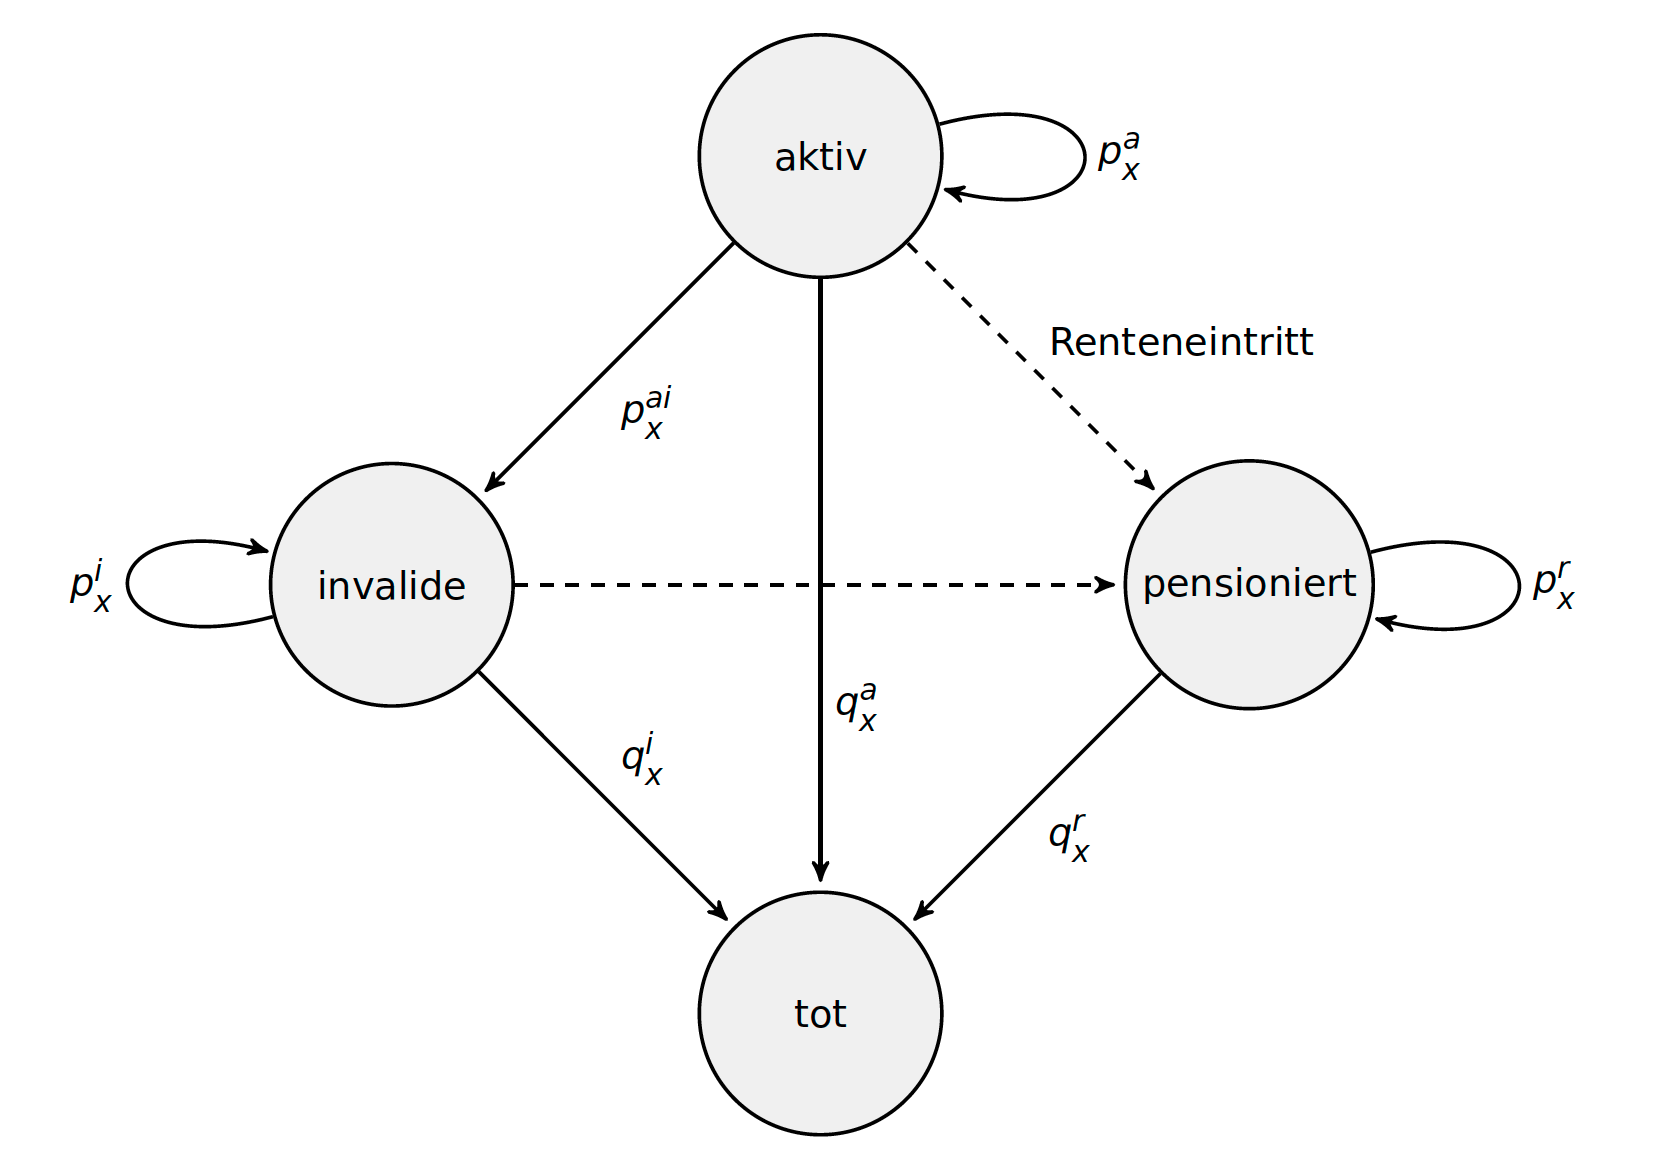
\includegraphics[width = .8\textwidth]{Bilder/ZustandsmodellPersVers}
\end{figure}
 \begin{itemize}
 	\item Modellannahmen nicht immer sachgerecht
 	\item Markov-Eigenschaft kritisch: Relevant, ob \textit{aktiv} $\rightarrow$ \textit{Rente} oder \textit{invalide} $\rightarrow$ \textit{Rente}
 	\item z.T. sehr viele Zustände erforderlich (z.B. Abhängigkeit der Leistungshöhe von Anzahl Dienstjahren, bei Invalidität der Zeitpunkt des Eintritts in den Invalidenstatus)
 	\item Markov in der Praxis begrenzt möglich, denn: Annahme der Markov-Eigenschaft oft kritisch, sehr viele Zustände zur Modellierung nötig, Erreichen des Gleichgewichtszustands fraglich
 \end{itemize}

\subsubsection{Risikoteilung}

\begin{itemize}
	\item teilweiser Risikotransfer im direkten Geschäft zwischen VN und Erstversicherer sowie im Rahmen von Rückversicherung (RV)
	\item Risikoteilung im Direktgeschäft: Selbstbehalt beim VN, genannt \textit{Franchisen}
	\item in der Rückversicherung: Selbstbehalt beim Erstversicherer, genannt \textit{Prioritäten}
	\item risikopolitisch und nicht gewinnorientierte Vorgehensweise
	\item für den Erstversicherer:
		\begin{itemize}
			\item Verringerung des versicherungstechnischen Risikos
			\item Erhöhung Zeichnungskapazität
			\item Solvenzverbesserung
			\item Kapitalkostenreduktion
		\end{itemize}
	\item für den Rückversicherer:
		\begin{itemize}
			\item Existenzgrundlage
			\item bessere Diversifikation der Risiken als beim Erstversicherer
		\end{itemize}
\end{itemize}

\subsubsection{Begrifflichkeiten Rückversicherung}
\begin{itemize}
	\item aktive RV: Angebot von Rückversicherungskaapzitäten
	\item passive RV: Nachfrage nach RV-Schutz durch Erstversicherer
	\item Retrozession: Weitergabe in Rückdeckung genommener Risiken eines RV an anderen RV
	\item obligatorische RV: Verpflichtung des Erstversicherers zur Übertragung aller vertraglich definierten Risiken ohne Ablehnungsrecht des RV
	\item fakultative RV: individuelle Abgabe und Annahme von Risiken auf einzelvertraglicher Basis
	\item Originalbasis: RV erhält anteilig Prämie und muss Deckungskapital bilden
	\item Risikobasis: RV erhält Risikobeitrag und bildet kein Deckungskapital
\end{itemize}

\subsubsection{Proportionale Risikoteilung}
\begin{itemize}
	\item proportionale Aufteilung der Schäden in festem Verhältnis zwischen Vertragspartnern
	\item Proportionen vorab fest und unabhängig von Schadenhöhen
	\item einfache Struktur, geringe Flexibilität
	\item bei RV Schicksalsteilung: Übernahme von Teilen des Erstversicherungsrisikos, aber nicht kaufmännischen oder unternehmerischen Risikos des Erstversicherers
	\item wichtigste Formen der proportionalen RV: Quotenrückversicherung, Summenexedentenrückversicherung
		\begin{itemize}
			\item QRV: feste Quotenabgabe $q$, Selbstbehalt $ \underbar{$S^{ind}$} = (1-q) \cdot S^{ind}$
			\item SERV: Festlegung eines Maximums $v_0$ als maximaler Selbstbehalt des Erstversicherers bei jedem einzelnen Risiko und vertragsindividuelle Quote $q_i = \frac{max\{v_i-v_0, \ 0\}}{v_i}$ in Abhängigkeit der jeweiligen Versicherungssumme
		\end{itemize}
	\item SERV dient der Homogenisierung des Portfolios und der Reduktion von Spitzenrisiken
	\item Üblicherweise Haftungsbegrenzung für RV i.H.v. Vielfachem $m$ von $v_0$. Mehrere aneinandergereiht, s.d. man Layering erhält.
\end{itemize}

\subsubsection{nicht-proportionale Risikoteilung}
\begin{itemize}
	\item alle, die keine proportionale Aufteilung vorsehen
	\item komplizierte Strukturen
	\item schwierige quantitative Analysierbarkeit
	\item gut zur Erreichung gezielter Effekte
	\item dominierend: Abzugsfranchise
		\begin{itemize}
			\item Franchisegrenze absoluter Höhe $a$ zwischen VN und VU
			\item Schaden in Höhe $X \ \Rightarrow \underbar{X}=min\{X,a\}$, d.h. VU übernimmt Teil, der $a$ übersteigt
			\item Jahresfranchise: analog mit Franchisegrenze und Jahresgesamtschaden
			\item Integralfranchise: wenn Grenze überschritten, übernimmt VU Schaden komplett
			\item Zeitfranchise: VN trägt jeden Schaden bis zum Ablauf der Frist selbst
		\end{itemize}
	\item wichtigste Formen: 
		\begin{itemize}
			\item Schadenexzedentenrückversicherung: Priorität $a$ und Limit $l$, Übernahme des Teils, der $a$ übersteigt und unter $l$ liegt. Wirkt pro Risiko, eignet sich für LCs. Limitierte Layer als Differenz zweier unlimitierter Layer darstellbar. 
			\item Kumulschadenexzedentenrückversicherung: Priorität $a^*$, Limit $l^*$ pro Kumulereignis (Anwendung auf Gesamtschäden von Kumulereignissen). Übernahme des die Prio übersteigenden Teils.
			\item Jahresüberschadenexzedentenrückversicherung: Anwendung auf Jahresgesamtschaden, ebenfalls Priorität und Limit
		\end{itemize}	
\end{itemize}

\subsubsection{Entschädigung}
\begin{itemize}
	\item Entschädigung $Z=g(X)$, $X \hat{=}$ Finanzaufwand, $g$ monoton wachsend, $g(x) \leq x$
	\item Selbstbehalt des VN $X-Z=X-g(X)$
	\item proportionale Selbstbeteiligung: $Z=g_1(X) \coloneqq q \cdot X, \ q \in (0,1)$
	\item Abzugsfranchise: $Z=g_2(X) \coloneqq (X-a)^+, \ a>0$
	\item Haftungsbegrenzung: $Z=g_3(X) \coloneqq min(X;I), \ I>0$
	\item allgemeine Darstellung der Entschädigung:
		\begin{equation}
			Z=q \cdot min\{(X-a)^+,I\}= \begin{cases}
				0 & X \leq a \\
				q \cdot (X-a) & a<X \leq a+I \\
				q \cdot I & a+i < X \\
			\end{cases}
		\end{equation}
	\item Prämie basiert auf Erwartungswert der Entschädigung $E(Z) \coloneqq E[q \cdot min \{(X-a)^+,I\}]= q \cdot \int_a^{a+I}(1-F(x))dx$, wobei $F(x)$ die Verteilungsfunktion der Finanzaufwände ist.
\end{itemize}













\chapter{Schadenversicheungsmathematik}

\subsubsection{Notation}
\begin{itemize}
\item $n$: Anzahl der Verträge
\item $\alpha_i$: Jahreseinheit des $i$-ten Vertrages, $i=1,...,n$
\item $v_i$: Versicherungssumme des $i$-ten Vertages
\item $b_i$: Jahresbeitrag des $i$-ten Vertrages
\item $N$: (zufällige )Anzahl Schäden
\item $X_j$: (zufällige) Höhe des $j$-ten Einzelschadens, $j=1,...,N$
\item $r$: Anzahl der Tarifmerkmale
\item $M_k$: $k$-tes Tarifmerkmal, $k=1,...,r$
\item $n_k$: Anzahl der verschiedenen Ausprägungen des $k$-ten Merkmals
\item $a_{j,k}$: $j$-te Ausprägung des $k$-Tarifmerkmals, $j=1,..., n_k$
\end{itemize}



\subsubsection{Schadenkennzahlen}
\begin{itemize}
\item Schadendaten: Zeitpunkt, Art und Ursache, Sachlicher Bezug, Ort, Entschädigung
\item Bestandsdaten: Versicherungssumme, persönliche Daten der VN, ...
\item Exposure: Das Risiko eines Vertrags oder eines Bestandes\\
Exposuremaß: versicherungstechnische Risiko bzw Schadenbedarf eines Bestandes (Bsp: Jahreseinheiten, Anzahl Risiken, Summe Beiträge, ...)
\item Anzahl Jahreseinheiten bzw. durchschnittliche Anzahl der Verträge: $n_0 := \sum_{i=1}^{n} \alpha_i$
\item Schadenhäufigkeit / Frequenz: $H:= \frac{\text{Anzahl Schäden}}{\text{Anzahl Jahreseinheiten}} = \frac{N}{n_0}$
\item Schadendurchschnitt: $D:= \frac{\text{Gesamtschaden}}{\text{Anzahl Schäden}} := \frac{\sum_{j=1}^N X_j}{N} = \frac{S}{N}$
\item Schadenbedarf: $SB:= \frac{\text{Gesamtschaden}}{\text{Anzahl Jahreseinheiten}} = \frac{S}{n_0} = H\cdot D = \text{Schadenhäufigkeit} \cdot \text{Schadendurchschnitt}$
\item Summe verdiente Beiträge: $b:= \sum_{i=1}^n \alpha_i \cdot b_i$
\item Schadenquote: $SQ:=\frac{\text{Gesamtschaden}}{\text{Summe verd. Beiträge}} = \frac{S}{b}$
\item durchschnittliche kumulierte Versicherungssumme: $v:= \sum_{i=1}^n \alpha_i \cdot v_i$
\item Schadensatz: $SS:=\frac{\text{Gesamtschaden}}{\text{durchschn. kumulierte V-Summe}} = \frac{S}{v}$
\item durchschnittliche Versicherungssumme: $v_0:= \frac{\text{durchschn. kumulierte V-Summe}}{\text{Anzahl Jahreseinheiten}} = \frac{v}{n_0}$
\item Schadengrad: $SG:=\frac{\text{Schadendurchschnitt}}{\text{durchschn. V-Summe}} = \frac{D}{v_0}$
\end{itemize}

\subsubsection{Gütekriterien Exposuremaß}
\begin{itemize}
\item Proportionalität zum Risiko
\item Praktikabilität
\item Zeitstabilität des Maßes
\end{itemize}

\subsubsection{Datentypen}
\begin{itemize}
\item Schadendaten: Zeitpunkt, Art und Ursache, Ort, Höhe der Entschädigung etc...
\item Bestandsdaten: Versicherungssumme, persönliche Daten etc...
\end{itemize}

\subsubsection{Grundlagen der Tarifierung}
\begin{itemize}
\item Risikomerkmal: statistisch signifikanter Zusammenhang zum Schadenverhalten
\item Tarifmerkmal: Rahmen der Tarifierung
\item Risikoklasse: genau die Risiken, die bei sämtlichen Tarifmerkmalen die gleiche Ausprägung haben
\end{itemize}
Vorgehen:
\begin{itemize}
\item Jedem Risiko wird im Rahmen der Tarifierung zunächst der Vektor der Ausprägung $(a_{i_1,1}, a_{i_2, 2}, ..., a_{i_r, r})$ der ausgewählten Tarifmerkmale $M_1,...,M_r$ zugeordnet. Dieser Vektor legt dann genau ein der $t:= \prod_{k=1}^r n_k=$Anzahl der Tarifzellen verschiedenen Tarifzellen eindeutig fest.
\item Für jedes $r$-Tupel $(i_1, ..., i_r)$ und damir für jede Tarifzelle ist die Nettorisikoprämie $b_{i_1, ..., i_r}$ zu bestimmen
\item Tarifmodelle verwenden Schadenbedarfe und für jedes Merkmal $M_k$, $k=1,...,r$ und jede Ausprägung $a_{j,k}$, $j=1,...,n_k$ dieses $k$-ten Merkmals einen der insgesamt $n:= \sum_{k=1}^r n_k$ sogenannten Marginalparameter
\item Dieses Marginalfaktoren bzw. summanden repräsentieren die verschiedenen Ausprägungen der Merkmale und quantifizieren den mittleren Einfluss der Ausprägung auf die Schadenaufwendungen und sind zu schätzen
\item $u_{k,j}:=$ Marginalfaktor bzw. summand der $j$-ten Ausprägung des $k$-ten Merkmals
\item Multiplikatives Modell: $b_{i_1, ..., i_r}:= sb\cdot \prod_{k=1}^r u_{k,i_k}$
\item Additives Modell: $b_{i_1, ..., i_r} := sb + \sum_{k=1}^r u_{k, i_k}$
\end{itemize}

\begin{figure}[ht]
	\centering
	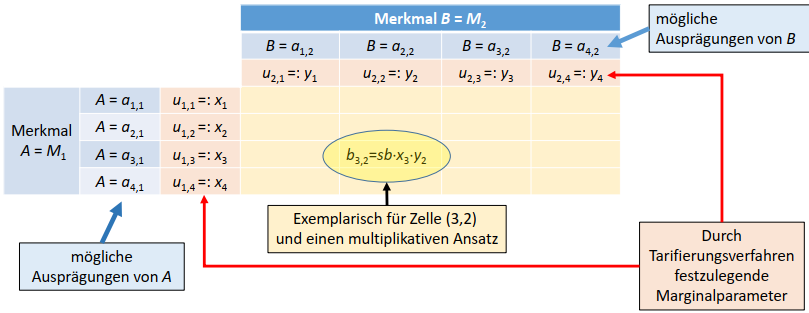
\includegraphics[width = .8\textwidth]{Bilder/Tarifierung2.png}
\end{figure}



\subsubsection{Tarifierungsverfahren}
Alles multiplikative Modelle: \\
Vereinfachte Bezeichnungen: $A:=M_1$, $B:=M_2$ Merkmale mit $p:=n_1$, $q:=n_2$ Merkmalsausprägungen. Es gilt: $t=p\cdot q$ und $n=p+q$. Außerdem: $x_i:=u_{1,i}, i=1, ...,p$ und $y_j:=u_{2,j}, j=1,...,q$. Zusätzlich $s_{i,j}$ Gesamtschaden in Tarifzelle $(i,j)$, $v_{i,j}$ Volumenmaß und $sb_{i,j}=\frac{s_{i,j}}{v_{i,j}}$ Schadenbedarf. \\
Es ergeben sich die Marginaldurchschnitt: $sb_{i,\circ}:=\frac{s_{i \bullet}}{v_{i\bullet}}$ und $sb_{\circ, j} := \frac{s_{\bullet j}}{v_{\bullet j}}$ und der Schadenbedarf $sb:=\frac{s_{\bullet \bullet}}{v_{\bullet \bullet}}$ \\

Tarifierungsverfahren mit Marginaldurchschnitten:
\begin{itemize}
\item heuristischer Ansatz: Marginalfaktoren als normierte Marginaldurchschnitte der Risiken mit den jeweiligen Merkmalsausprägungen definieren:\\
$x_i^{MD} := \frac{sb_{i\circ}}{sb}$ \\
$y_j^{MD} := \frac{sb_{\circ j}}{sb}$ 
\item Dann folgt: $b_{i,j}^{MD} := sb \cdot x_i^{MD} \cdot y_j^{MD}$
\item Verfahren liefert meist wenig zufriedenstellende Ergebnisse $\rightarrow$ Weiterentwicklung erforderlich
\end{itemize}
Tarifierungsverfahren von Bailey $\&$ Simon:
\begin{itemize}
\item Ansatz orientiert sich an der Abstandsfunktion des $\chi^2$-Tests
\item Versucht die Marginalfaktoren $x_i$, $y_j$ so zu wählen, dass die Summe der (gewichteten) quadratischen Abstände zwischen den beobachteten Gesamtschäden $s_{ij}$ und den kumulierten Nettorisikoprämien $v_{i,j}\cdot b_{i,j} = v_{i,j}\cdot sb \cdot x_i \cdot y_j$ über alle Zellen minimiert wird.
\item Lösungen ergeben sich - nach Nullsetzen der partiellen Ableitungen - durch "p+q nichtlinearen Bestimmungsgleichungen" (nicht explizit lösbar, aber lösbar mit Fixpunktiteration)
\item Grenzwerte der Iteration geben die Marginalfaktoren $x_i^{BS}$ und $y_j^{BS}$ (nicht eindeutig bestimmt)
\item Es folgt: $b_{i,j}^{BS} := sb \cdot x_i^{BS} \cdot y_j^{BS}$
\item Verfahren reagiert empfindlich auf Ausreißer und überschätzt beobachteten Gesamtschaden
\end{itemize}
Marginalsummenverfahren
\begin{itemize}
\item Ansatz: Für jede Ausprägung eines der beiden Merkmale sollen die kumulierten Nettorisikoprämien mit den kumulierten Gesamtschäden übereinstimmen.
\item Grundlage zur Bestimmung der Marginalfaktoren sind Marginalsummengleichungen 
\item Marginalsummengleichungen ergeben nichtlineares Gleichungssystem mit $p+q$ Gleichungen und Unbekannten
\item Lösen ebenfalls mit Fixpunktiteration:
\begin{align}
x_i = \frac{s_{i\bullet }}{sb \cdot \sum_{j=1}^q v_{i,j} \cdot y_j} \\
x_i = \frac{s_{i \bullet}}{sb \cdot \sum_{j=1}^q v_{i,j} \cdot x_i}
\end{align}
\item Bei Konvergenz ergeben sich die Grenzwerte als Marginalfaktoren $x_i^{MS}$ und $y_j^{MS}$
\end{itemize}



\subsubsection{Auswahl der Tarifmerkmale}
\begin{figure}[ht]
	\centering
	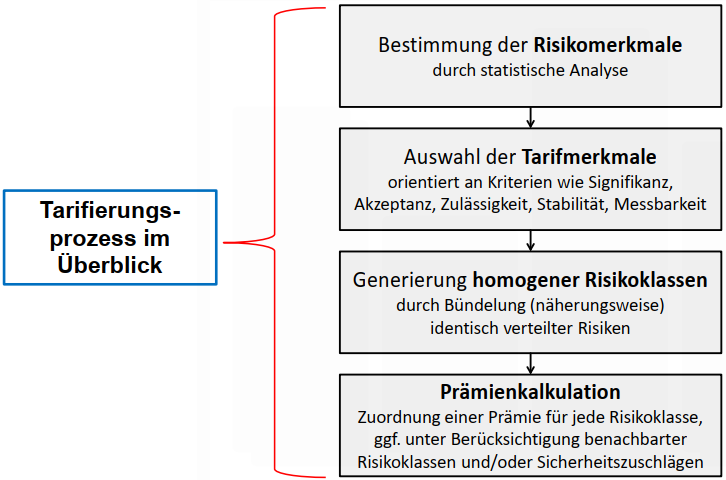
\includegraphics[width = .8\textwidth]{Bilder/Tarifierung.png}
\end{figure}
1. Ermittlung von Risikomerkmalen
\begin{itemize}
\item Finden von statistisch signifikanten Merkmalen aus Daten zweierlei Arten: Schadendaten und Bestandsdaten
\item Auswahl potenzieller Risikomerkmale permanent prüfen
\item Besondere Beachtung der Großschäden durch "Kupierung": Schäden werden an sog. Kuperungsgrenzen abgeschnitten. Pro Schaden stellt die Grenze die max. Höhe dar, mit denen Schadenaufwendungen in den weiteren Analysen berücksichtigt werden
\end{itemize}
2. Auswahlkriterien einzelner Tarifmerkmale
\begin{itemize}
\item Wichtigste Kriterien: Signifikanz, möglichst unabhängig, Zulässigkeit, Messbarkeit, Anzahl der Tarifmerkmale, Stabilität/Robustheit, Bezug zum Risiko, Imageaspekte
\end{itemize}
3. Auswahlmethoden der Gesamtheit der Tarifmerkmale
\begin{itemize}
\item Einerseits: Gute Erklärung des Schadenaufkommens, andererseits: stochastische Unabhägigkeit oder Analysierung ihrer Wechselwirkung
\item Für die Tarifmerkmale gemeinsame Verteilung: $P^{X_1,...,X_r}$
\item Bei stochastischer Abhängigkeit steigt der Grad der Komplexität um $P$ zu berechnen deutlich an
\item Moderne Ansätze: Einsatz von Copulas für die Abhängigkeiten
\item Ansatz 1: Multiple Regressionsanalyse (\textbf{GENAUER? Kap 4})
\item Ansatz 2: Verfahren der schrittweisen Auswahl (\textbf{GENAUER?})
\end{itemize}


\subsubsection{Abwicklungsmuster}

Abwicklungsmuster sind die Basis der Modellbildung für zahlreiche
Methoden der Schadenreservierung. Sie unterstellen für ausgewählte zentrale Kennzahlen der Schadenabwicklung bestimmte Systematiken und erklären
die Abweichungen von diesen systematischen Größen (Erwartungswerten) als
zufällige und unsystematische Schwankungen

1. für Anteile $\vartheta$
\begin{itemize}
\item Für jedes Anfalljahr $i$ wird der erwartete Zuwachs im $k$-ten Abwicklungsjahr im Verhältnis zum erwarteten Endschadenstand definiert: $\vartheta_k = \frac{E[Z_{i,k}]}{E[S_{i,n}]}$, $i,k=0,...,n$ (Anteile unabhängig von Anfalljahr)
\item Es gilt $\sum_{k=0}^n =1$.
\item Bei Schadenanzahl bzw. -zahlungen gilt: $\vartheta_k >0$
\end{itemize}
2. für Quoten $\gamma$
\begin{itemize}
\item Für jedes Anfalljahr $i$ wird der erwartete Schadenstand im $k$-ten Abwicklungsjahr im Verhältnis zu dem erwarteten Endschadenstand definiert: $\gamma_k = \frac{S[Z_{i,k}]}{E[S_{i,n}]}$, $i,k=0,...,n$ (Quoten unabhängig von Anfalljahr)
\item Es gilt $\gamma_n=1$
\item Bei Schadenanzahl bzw. -zahlungen gilt: $\gamma_0 < ... < \gamma_n$
\end{itemize}
3. Für Faktoren $\varphi$
\begin{itemize}
\item Für jedes Anfalljahr wird der erwartete Schadenstand im $k$-ten Abwicklungsjahr im Verhältnis zum erwarteten Schadenstand im $(k-1)$-ten Abwicklungsjahr definiert: $\varphi_k = \frac{S[S_{i,k}]}{E[S_{i,k-1}]}$, $i,k=0,...,n$
\item $\hat{\gamma}_k = \prod_{l=k+1}^n \frac{1}{\hat{\varphi}_l}$
\item Bei Schadenanzahl bzw. -zahlungen gilt: $\varphi_k >1$
\end{itemize}
4. Für Schadenquotenzuwächse
\begin{itemize}
\item In Anwendung verwendet man die Prämieneinnahmen der Anfalljahre für Volumenmaße $\pi_0,..., \pi_n$
Erwarteter Schadenquotenzuwachs des $k$-ten Abwicklungsjahrs für das $i$-te Anfalljahr: $\frac{E[Z_{i,k}]}{\pi_i}$, $i,k=0,...,n$
\item erwartete Endschadenquote: $\frac{E[S_{i,n}]}{\pi_i}$
\end{itemize}

\subsubsection{GLMs}
\begin{itemize}
\item Verallgemeinerte lineare Modelle erweitern den Ansatz der linearen Regression durch Verwendung einer streng monoton wachsenden Transformation $g: \mathbb{R} \rightarrow \mathbb{R}$ -> "Link-Funktion"
\item transformierter Erwartungswert soll lineare Funktion in $x$ sein:
\begin{equation}
g(\mu(x)) = g(E[Y|X=x]) = a_0 + \sum_{i=1}^r a_i \cdot x_i = \eta (x)
\end{equation}
\item $\eta(x)$ wird auch linearer Prädiktor genannt
\item Durch inverse Link-Funktion: $\mu(x) = g^{-1}(\eta(x))$
\item Zugehöriges GLM lautet:
\begin{equation}
Y=g^{-1} \left( a_0 + \sum_{i=1}^r a_i \cdot X_i \right) +\widetilde{\varepsilon}
\end{equation}
\item log-lineares Modell: $\mu(x) = e^{a_0 + \sum_{i=1}^r a_i \cdot x_i} = e^{\eta (x)} >0$ 
\item Beziehung zu Marginalsummenverfahren: Für genau zwei Merkmale und den Ansatz Poisson-verteilter Schadenaufwände überführt den log-link-Ansatz das ursprüngliche Poisson-Modell in das Marginalsummenverfahren 
\end{itemize}




\subsubsection{Basisverfahren der Schadenreservierung}

Chain-Ladder-Verfahren
\begin{itemize}
\item Chain-Ladder Faktoren:
\begin{equation}
\hat{\varphi}_k^{CL} := \frac{\sum_{j=0}^{n-k} S_{j,k}}{\sum_{j=0}^{n-k} S_{j,k-1}}= \sum_{j=0}^{n-k} \frac{S_{j,k-1}}{\sum_{h=0}^{n-k} S_{h,k-1}} \cdot \frac{S_{j,k}}{S_{j,k-1}}, k=1,...,n
\end{equation}
\item Alle beobachtbaren Schadenstände werden verwendet (sonst nichts)
\item Die aktuellen Schadenstände $S_{i,n-i}$, $i=0,...,n$, aus der Diagonale des Abwicklungsdreiecks mit Hilde der Chain-Ladder-Faktoren sukzessive auf das Niveau der späteren Abwicklungsjahre hochgerechnet.
\item Ergebnisse werden als Chain-Ladder-Prädiktoren bezeichnet:
\begin{equation}
\hat{S}_{i,k}^{CL}:= \hat{\varphi}_k^{CL} \cdot \hat{S}_{i,k-1}^{CL}
\end{equation}
\item Reserven für Anfalljahr $i$ ergeben sich aus der Differenz der Prädiktoren für den erwarteten Entschadenstand und dem aktuellen Schadenstand:
\begin{equation}
\hat{R}_i^{CL}:= \hat{S}_{i,n}^{CL} - S_{i,n-i}
\end{equation}
\end{itemize}
Loss-Development-Verfahren
\begin{itemize}
\item Stellt ein Abwicklungsmuster für Quoten und dass für diese Quoten $\gamma_0, ...,\gamma_n$ a-priori-Schätzer $\hat{\gamma}_0, ..., \hat{\gamma}_n$ unterliegen 
\item Aktuelle Schadenstände $S_{i, n-i}$ per Division durch Schätzer auf Niveau des letzten Abwicklungsjahr hochgerechnet und mit Faktor $\hat{\gamma}_k$ auf Niveau des $k$-ten Abwicklungsjahrs zurück skaliert:
\begin{equation}
\hat{S}_{i,k}^{LD} := \hat{Y}_k \cdot \frac{S_{i,n-i}}{\hat{Y}_{n-i}}
\end{equation}
\end{itemize}
Bornhuetter-Ferguson-Verfahren
\begin{itemize}
\item Ähnlich wie LD-Verfahren, aber zusätzlich zu a-priori Schätzer $\hat{\gamma}_0, ..., \hat{\gamma}_n$ für Quoten noch a-priori-Schätzer $\hat{\alpha}_0, ..., \hat{\alpha}_n$ für erwartete Schadenstände ($\alpha_i := E[S_{i.n}]$)
\item aktuelle Schadenstände mit Hilfe der a-priori Schätzer linear fortgeschrieben.
\begin{equation}
\hat{S}_{i,k}^{BF} := S_{i,n-i}+(\hat{\gamma}_k-\hat{\gamma}_{n-i})\cdot \hat{\alpha_i}
\end{equation}
\item Durch Differenzbildung werden die BF-Prädiktoren für Zuwächste errechnet:
\begin{equation}
\hat{Z}_{i,k}^{BF} := \hat{S}_{i,k}^{BF} - \hat{S}_{i,k-1}^{BF} = (\hat{\gamma}_k - \hat{\gamma}_{k-1}) \cdot \hat{\alpha}_i
\end{equation}
\item iteriertes Bornhuetter-Ferguson-Verfahren: Nach der ersten Anwendung werden die Prädiktoren $\hat{S}_{i,n}^{BF}$ anstatt der $\hat{\alpha}_i$ verwendet (Einfluss wird so reduziert). Verfahren wird so lange wiederholt bis sich Grenzwerte einstellen als Prädiktoren
\end{itemize}
Additives Verfahren/ Incremental-Loss-Ratio-Verfahren
\begin{itemize}
\item Basiert auf Annahme, dass es Volumenmaße $\pi_0, ..., \pi_n$ für die Anfalljahre $i=0,...,n$ gibt.
\item Außerdem Abwicklungsmuster für die erwarteten (Schaden-)Quoten-Zuwächse $\frac{E[Z_{i,k}]}{\pi_i}$, sodass es Parameter $\zeta_0,...,\zeta_n$ gibt mit $\zeta_k=\frac{E[Z_{i,k}]}{\pi_i}$
\item Schätzer für relative Zuwächse werden additive Schadenquotenzuwächse verwendet:
\begin{equation}
\zeta_k^{AD} := \frac{\sum_{j=0}^{n-k} Z_{j,k}}{\sum_{j=0}^{n-k} \pi_j} = \sum_{j=0}^{n-k} \frac{\pi_j}{\sum_{h=0}^{n-k} \pi_h} \cdot \frac{Z_{j,k}}{\pi_j}
\end{equation}
\item Schätzer setzen für den Zuwachs des $k$-ten Abwicklungsjahr die Summe sämtlicher Zuwächse im $k$-Abwicklungsjahr zur Summe der zugehörigen Volumenmaße
\item Mit diesen Schätzern erhält man Prädiktoren für Zuwächse und Schadenstände:
\begin{align}
\hat{Z}_{i,k} := \pi_i \cdot \hat{\zeta}_k^{AD} \\
\hat{S}_{i,k}^{AD} := S_{i,n-i} + \sum_{j=n-i+1}^k \hat{Z}_{i,j}^{AD}
\end{align}
\end{itemize}
Cape-Cod-Verfahren
\begin{itemize}
\item Wie Additives Verfahren Volumenmaße $\pi_0,...,\pi_n$. Zusätzlich a-priori-Schätzer $\hat{\gamma}_0,...,\hat{\gamma}_n$ für Quoten
\item Annahme: erwartete Schadenquoten unabhängig von Anfalljahr $i$, daher existiert Parameter $\kappa$: $\frac{E[S_{i,n}]}{\pi_i}=\kappa$
\item $\kappa$ wird geschätzt:
\begin{equation}
\hat{\kappa}^{CC} = \frac{\sum_{j=0}^n S_{j,n-j}}{\sum_{j=0}^n \hat{\gamma}_{n-j} \cdot \pi_j} = \sum_{j=0}^n \frac{\hat{\gamma}_{n-j} \cdot \pi_j}{\sum_{h=0}^n \hat{\gamma}_{n-h} \cdot \pi_h} \cdot \frac{S_{j,n-j}}{\hat{\gamma}_{n-j}\cdot \pi_j}
\end{equation}
\item Cape-Code-Prädiktoren: 
\begin{equation}
\hat{S}_{i,k}^{CC} := S_{i,n-i} + (\hat{\gamma}_k - \hat{\gamma}_{n-i}) \cdot \pi_i \cdot \hat{\kappa}^{CC}
\end{equation}
\end{itemize}
Alle Verfahren sind Spezialfälle von Bornhuetter-Ferguson-Verfahrens. Unterschieden nur durch die Schätzung der Parameter.
\begin{figure}[ht]
	\centering
	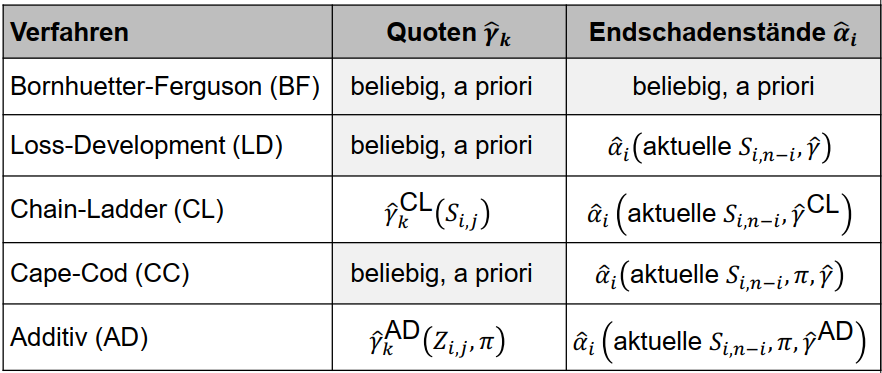
\includegraphics[width=.8\textwidth]{Bilder/Abwicklungsverfahren.png}
\end{figure}
\begin{figure}[ht]
	\centering
	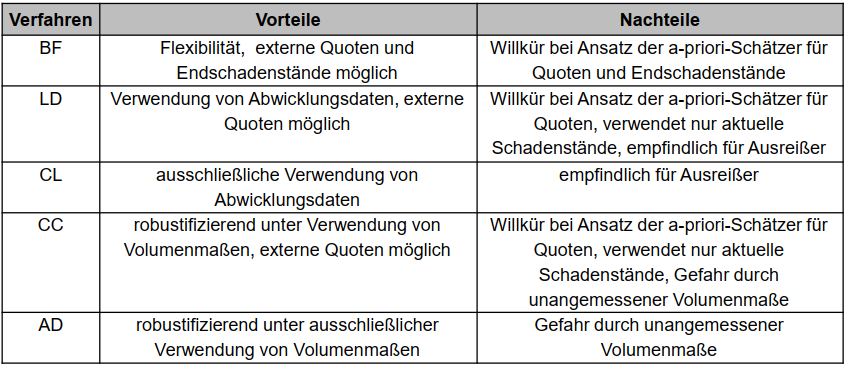
\includegraphics[width=\textwidth]{Bilder/Abwicklungsverfahren_PundC.png}
\end{figure}



\newpage
\subsubsection{Erweiterung der Basisverfahren}
1. Ausreißereffekte \\
Besser, wenn a-priori-Schätzer vorhanden. Daher Chain-Ladder sehr anfällig und Cape-Cod am besten

2. Inflation\\
Separationsverfahren bietet Möglichkeit, Kalendereffekte zu berücksichtigen und eine Art Inflationsvereinigung vorzunehmen. Kurze Zusammenfassung: Es gibt Parameter für Abwicklungsjahre und für Kalenderjahre und für die Zuwächse gilt: $E[Z_{i,k}]=v_i\cdot \gamma_{i+k}\cdot \vartheta_k$. Schätzung der Parameter durch Marginalsummengleichungen. Durch bspw. Extrapolation Schätzung der Inflationparameter der nächsten Jahre. Am Ende: $\hat{Z}_{i,k}= v_i \cdot \hat{\gamma}_{i+k} \cdot \hat{\vartheta}_k$ 

3. Nachlauf\\
Annahme: Schäden innerhalb von $n+1$ Jahren vollständig abgewickelt. In Ausnahmefällen noch nach dem $n$-ten Jahr Änderungen in Schadenständen -> "Nachlauf" 

















\chapter{Personenversicherungsmathematik}

\begin{figure}[ht]
	\centering
	
\includegraphics[width=.8\textwidth]{Bilder/Korbinian.png}
\end{figure}

\subsubsection{Modell}
\begin{itemize}
	\item h Ereignisse bzgl. einer Person, das zuerst eintretende Ereignis führt zum Ausscheiden aus Gesamtheit
	\item $h$: Anzahl der Ausscheideursachen, $T_i$ Zeitpunkt Eintritt des Ereignisses $i$, $X_i$ Alter bei Eintritt des Ereignisses $i$
	\item $X_i = T_i-t^*$, $t^* \hat{=}$ Geburtszeitpunkt, $G \coloneqq \lfloor t^* \rfloor$ das Geburtsjahr
	\item $X\coloneqq min\{X_i\}$ Ausscheidealter, $U\coloneqq min\{i \in \{1,...,h\}:X_i=X\}$: Ausscheideursache
	\item $\tensor[_{1}]{q}{}_x^{(i)}(G)$: Wahrscheinlichkeit einer $x$-jährigen Person der HGSH mit Geburtsjahr $G$ innerhalb des Zeitintervalls $(x,x+1)$ mit der Ursache $i$ auszuscheiden. Verbleibewahrscheinlichkeit $p_x \coloneqq 1-q_x$
	\item Allgemein: 
	\begin{align}
		\tensor[_{s}]{q}{}_x(G)\coloneqq \mathbb{P}[X \leq x+s | X>x] \\
		\tensor[_{s}]{p}{}_x(G) \coloneqq 1-\tensor[_{s}]{q}{}_x(G) = \mathbb{P}[X>x+s|X>x]
	\end{align}
	\item mehrjährige Verbleibewahrscheinlichkeit (noch mind. $k$ Jahre in HGSH verbleiben): $\tensor[_{k}]{p}{}_x = \prod_{j=0}^{k-1}p_{x+j}$
	\item Zwillingsfreiheit: nur eine Ausscheideursache führt zum Ausscheiden.
	\item Zyklenfreiheit: keine Übergänge von Nebengesamtheit in Hauptgesamtheit
\end{itemize}

\subsubsection{Typische Rechnungsgrundlagen}
\begin{itemize}
	\item biometrische Rechnungsgrundlagen / Ausscheideordnung
	\item Rechnungszins
	\item Kosten
	\item Rechnungsgrundlage 1. Ordnung: vorsichtig, inkl. Sicherheit
	\item Rechnungsgrundlage 2. Ordnung: Erwartungswert, keine Sicherheiten
\end{itemize}

\subsubsection{Risikomerkmale von Ausscheidewahrscheinlichkeiten}
\begin{itemize}
	\item Eigenschaften, die in statistisch überprüfbarer Weise mit dem Erwartungswert zusammenhängen
	\item gleichzeitig mehrere Merkmale von Bedeutung (eines reicht nicht)
	\item Annahme: Ausscheidewahrscheinlichkeit hängt nur von den Merkmalen ab
	\item vieles wird nicht berücksichtigt
\end{itemize}

\subsubsection{Kosten}
\begin{itemize}
	\item Kostenarten: Abschluss ($\alpha$), Inkasso ($\beta$), Verwaltung ($\gamma$)
	\item Unterschieden werden proportionale (bezogen auf Beitrag oder VS) und Stückkosten
\end{itemize}

\subsubsection{Erfüllungsbetrag}
\begin{itemize}
	\item Der Erfüllungsbetrag einer ungewissen Verpflichtung $B$ ist extensional definiert durch die Menge seiner Realisierungen $b_m \coloneqq \sum_n v^{t_n^{(m)}}s_n^{(m)}$ für $m=0,1,..$, d.h. die Menge der finanzmathematischen Barwerte der ungewissen Verpflichtung.
\end{itemize}

\subsubsection{Leistungsbarwert}
\begin{itemize}
	\item Barwert der Gesamtverpflichtung gegenüber einer Person: 
	\begin{equation}
		\tensor[_{0}]{B}{}_x^{L}= \sum_{k\geq 0}v^k \tensor[_{k}]{p}{}_x \tensor[_{k}]{\hat{L}}{}_x
	\end{equation}
	\begin{equation}
		\tensor[_{k}]{\hat{L}}{}_x \coloneqq	\tensor[_{k}]{L}{}_x^{(0)}+\sum_{i=1}^h \tensor[_{k}]{L}{}_x^{(i)}q_{x+k}^{(i)}, \ k = 0,1,...
	\end{equation}
	\item $\tensor[_{k}]{\hat{L}}{}_x$: Erwartungswert der gesamten Leistung, die durch Erreichen des Altersintervalls $]x+k,x+k+1[$ ausgelöst werden kann, diskontiert auf Beginn des Jahres
	\item $\tensor[_{k}]{L}{}_x^{(0)}$: Erwartungswert der Leistungen, die durch Erreichen des Alters $x+k$ in der Hauptgesamtheit verursacht werden, diskontiert auf Jahresbeginn
	\item $\tensor[_{k}]{L}{}_x^{(i)}$: Erwartungswert der Leistungen, die durch das Ausscheiden im Jahr $]x+k, x+k+1[$ aus der Ursache $i$ verursacht werden, soweit nicht durch $\tensor[_{k}]{L}{}_x^{(0)}$ erfasst, diskontiert auf Jahresbeginn
	\item Leistungsbarwert zum Alter $x+m$:
	\begin{equation}
		\tensor[_{m}]{B}{}_x^{L}=\sum_{k\geq0}v^k \tensor[_{k}]{p}{}_{x+m} \tensor[_{m+k}]{\hat{L}}{}_x, \ \ \  m=0,1,...
	\end{equation}
\end{itemize}

\subsubsection{Prämienbarwerte}
\begin{itemize}
	\item Prämienbarwert zum Alter $x$ gegenüber einer Person:
	\begin{equation}
		\tensor[_{0}]{B}{}_x^{P} = \sum_{k \geq 0} v^k \tensor[_{k}]{p}{}_x \tensor[_{k}]{\hat{P}}{}_x
	\end{equation}
	\item $\tensor[_{k}]{\hat{P}}{}_x$: Erwartungswert der Prämienleistung des Jahres $]k,k+1]$, die durch Erreichen des Alters $x+k$ in der Hauptgesamtheit verursacht werden, diskontiert auf Jahresbeginn
	\item Prämienbarwert zum Alter $x+m$: $\tensor[_{m}]{B}{}_x^P = \sum_{k \geq 0}v^k \tensor[_{k}]{p}{}_{x+m} \tensor[_{k+m}]{\hat{P}}{}_x, \ \ m =0,1,...$
\end{itemize}

\subsubsection{Reserven}
\begin{itemize}
	\item Prospektive Reserve $\tensor[_{m}]{V}{}_x^{pro}$: Betrag, der zum jeweiligen Stichtag verfügbar sein muss, um Vertrag im Mittel zu erfüllen
	\item Retrospektive Reserve $\tensor[_{m}]{V}{}_x^{retro}$: Betrag, der rechnungsmäßig nach Abrechnung von Einnahmen und Ausgaben noch vorhanden ist
	\item Nach $m$ Jahren soll die Differenz zwischen Barwert zukünftiger Leistungen und Barwert zukünftiger Prämien durch die Reserve gedeckt sein: 
	\begin{equation}
		\tensor[_{m}]{V}{}_x^{pro} = \tensor[_{m}]{B}{}_x^{L} - \tensor[_{m}]{B}{}_x^{P} = \sum_{k \geq 0} v^k \tensor[_{k}]{p}{}_{x+m}(\tensor[_{m+k}]{\hat{L}}{}_x - \tensor[_{m+k}]{\hat{P}}{}_x)
	\end{equation}
	\begin{equation}
		\tensor[_{m}]{V}{}_x^{retro} = \frac{1}{v^m \tensor[_{m}]{p}{}_x} \left[K+\sum_{k=0}^{m-1}v^k \tensor[_{k}]{p}{}_x (\tensor[_{k}]{\hat{P}}{}_x - \tensor[_{k}]{\hat{L}}{}_x) \right]
	\end{equation}
	\begin{equation}
		\tensor[_{m}]{V}{}_x^{pro} - \tensor[_{m}]{V}{}_x^{retro} = \frac{1}{v^m \tensor[_{m}]{p}{}_x} \left(\tensor[_{0}]{V}{}_x^{pro} - \tensor[_{0}]{V}{}_x^{retro}\right)
	\end{equation}
\end{itemize}

\subsubsection{Versicherungsmathematische Bilanzgleichung}
\begin{itemize}
	\item $\tensor[_{m}]{V}{}_x + \tensor[_{m}]{\hat{P}}{}_x = \tensor[_{m}]{\hat{L}}{}_x + vp_{x+m} \ \tensor[_{m+1}]{V}{}_x$
	\item Spar- und Risikoprämie: 
		\begin{align}
			\tensor[_{m}]{V}{}_x + \tensor[_{m}]{\hat{P}}{}_x &= \tensor[_{m}]{P}{}_x^S + \tensor[_{m}]{P}{}_x^R \\
			\Leftrightarrow \tensor[_{m}]{\hat{P}}{}_x &= v \cdot \tensor[_{m+1}]{V}{}_x - \tensor[_{m}]{V}{}_x + \tensor[_{m}]{\hat{L}}{}_x - v \cdot q_{x+m} \cdot \tensor[_{m+1}]{V}{}_x
		\end{align}
\end{itemize}

\chapter{Pensionenversicherung}
\subsubsection{Bevölkerungsmodell - Ausscheidewahrscheinlichkeiten q und Verbleibewahrscheinlichkeiten p}

\begin{figure}[ht]
	\centering
	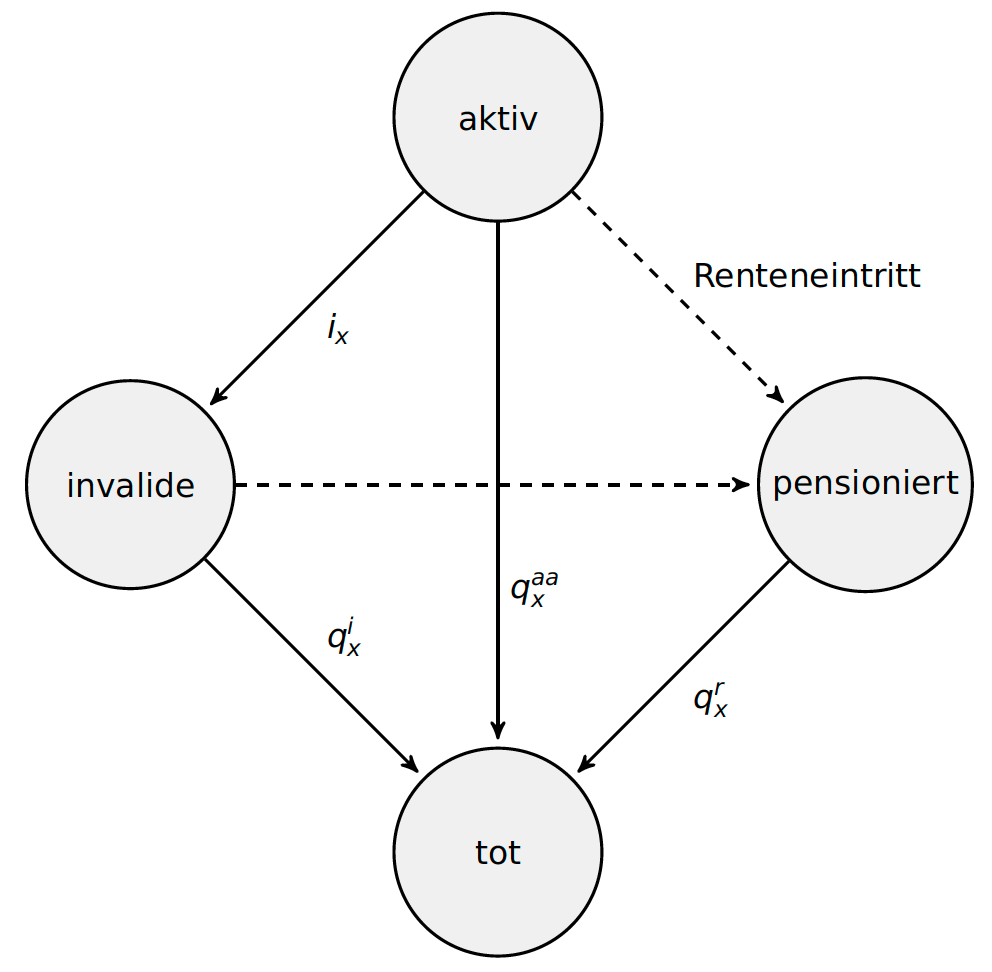
\includegraphics[width=.75\textwidth]{Bilder/Bevoelkerungsmodell.png}
\end{figure}

\begin{figure}[ht]
	\centering
	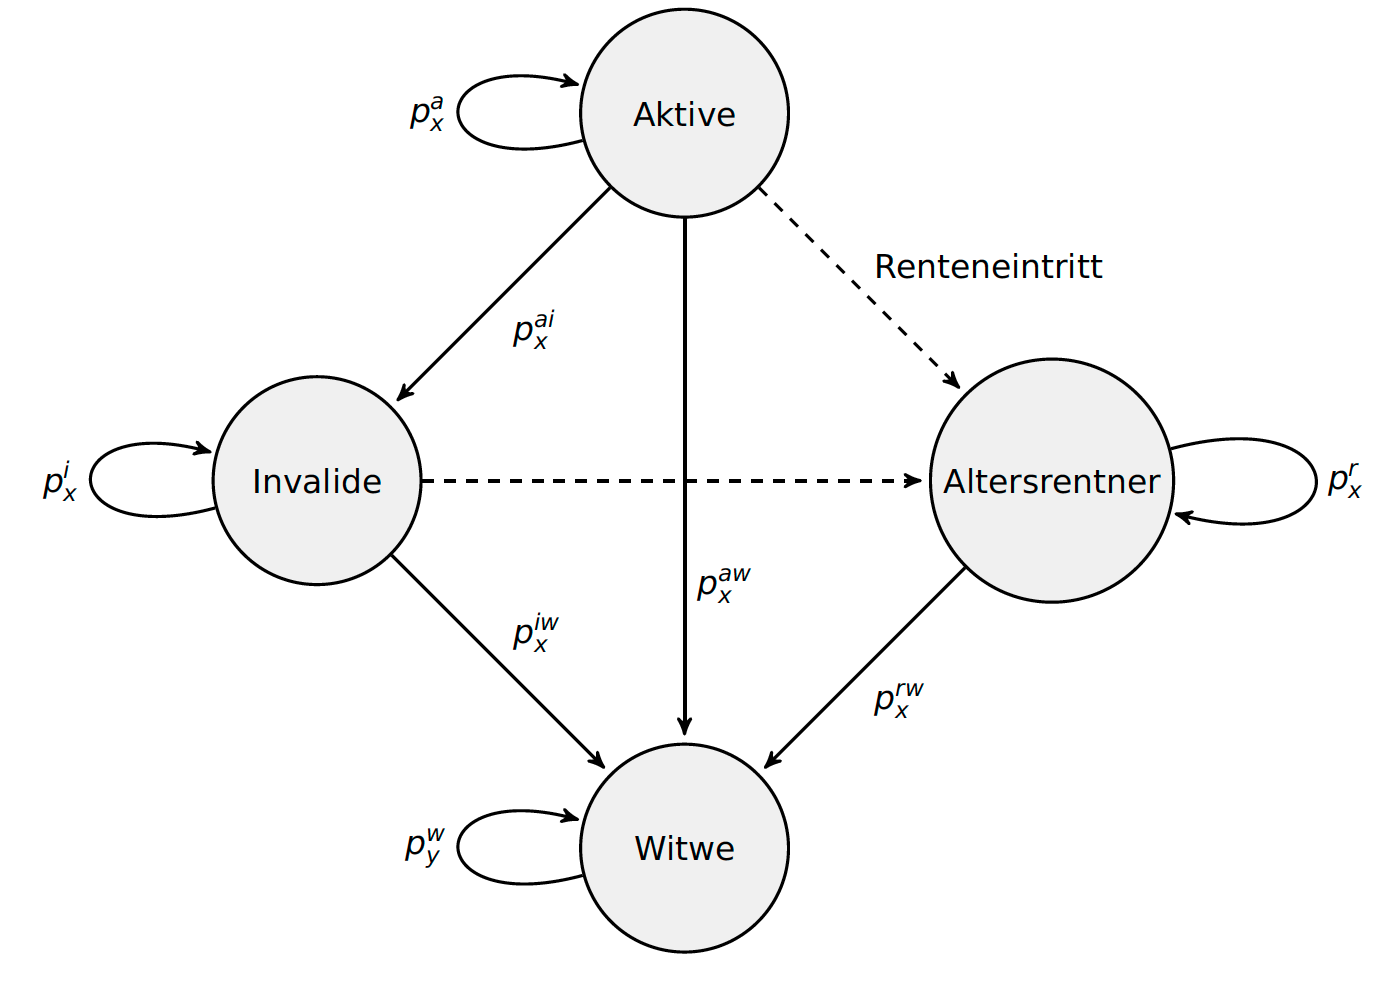
\includegraphics[width=.75\textwidth]{Bilder/Bevoelkerungsmodell2.png}
\end{figure}

\subsubsection{Rechnungsgrundlagen - Steuerbilanz / Handelsbilanz}
\begin{itemize}
	\item Fluktuation: Ausscheiden eines Mitarbeiters ohne Versorgungsfall (Kündigung)
	\item Steuerbilanz: Zinssatz 6$\%$ vorgeschrieben, liegt über durchschnittlichem Marktzins der letzten 10 Geschäftsjahre $\Rightarrow$ Unterbewertung der Verpflichtungen
	\item Steuerbilanz: künftige Erhöhungen nur einbeziehbar, wenn sie dem Grunde und der Höhe nach feststehen
	\item Handelsbilanz: bestmögliche Schätzung vornehmen $\Rightarrow$ Unterbewertung in steuerbilanzieller Bewertung
	\item Berechnung Deckungsrückstellung regulierte Pensionskassen:
		\begin{itemize}
			\item Rechnungsgrundlagen vorsichtig wählen, Sicherheitszu-/abschläge
		\end{itemize}
\end{itemize}

\subsubsection{Leistungsbarwerte}

\begin{itemize}
	\item Barwert einer Verpflichtung ggü. $x$-jähriger Person: $\tensor[_{0}]{B}{}_x^L=\sum_{k\geq 0}v^k \cdot \tensor[_{k}]{p}{}_x \cdot \tensor[_{k}]{\hat{L}}{}_x$
	\item $\tensor[_{k}]{\hat{L}}{}_x$: EW der gesamten Leistung, die durch Erreichen des Altersintervalls $(x+k, \ x+k+1]$ ausgelöst wird.
\end{itemize}

\subsubsection{Barwert einer lebenslänglich laufenden Rente, jährlich $t$ Raten mit Betrag $1/t$ vorschüssig zahlbar}
\begin{equation}
	\tensor[^{(t)}]{\text{\textit{ä}}}{}_x^r=\sum_{k \geq 0} v^k \cdot \tensor[_{k}]{p}{}_x^r \cdot  \tensor[_{k}^{(t)}]{\hat{L}}{}_x^r
\end{equation}
\begin{equation}
	\tensor[_{k}^{(t)}]{\hat{L}}{}_x^r \text{: Barwert der Rentenzahlung des Alters } (x+k, x+k-1] \text{ zum Beginn des Jahres}
\end{equation}

\subsubsection{Barwert einer über die Aktivenzeit laufenden Rente, Jahresbeitrag 1, vorschüssig zahlbar in $t$ Raten p.a.}
\begin{equation}
	\tensor[^{(t)}]{\text{\textit{ä}}}{}_x^a=\sum_{k = 0}^n v^k \cdot \tensor[_{k}]{p}{}_x^a \cdot  \tensor[_{k}^{(t)}]{\hat{L}}{}_x^a
\end{equation}

 \subsubsection{Invarianzsatz}
 \begin{itemize}
 	\item  Auf der Basis des Axiomensystems hängen Anwartschaftsbarwerte von Renten mit gleichbleibender Rentenhöhe nicht von der Zahlungsweise ab, wenn sowohl der Zeitpunkt des die Rente auslösenden Ereignisses als auch der Zeitpunkt des die Rente beendigenden Ereignisses innerhalb eines Jahres gleichverteilt sind.
 	\item Anwartschaft eines Aktiven auf lebenslängliche Invalidenrente: $\tensor[^{(t)}]{\text{\textit{ä}}}{}_x^{ai} = \text{\textit{ä}}_x^{ai}$
 \end{itemize}

\subsubsection{Barwert der Anwartschaft eines Aktiven des Alters $x$ auf lebenslänglich laufende Invalidenrente, Jahresbetrag 1, vorschüssig in $t$ Raten p.a. zahlbar}
\begin{equation}
	\tensor[^{(t)}]{\text{\textit{ä}}}{}_x^{ai}=\text{\textit{ä}}_x^{ai}=\sum_{k = 0}^n v^k \cdot \tensor[_{k}]{p}{}_x^a \cdot  \tensor[_{k}^{(t)}]{\hat{L}}{}_x^{ai}
\end{equation}

\subsubsection{Barwert der Anwartschaft eines Aktiven des Alters $x$ auf lebenslänglich laufende Altersrente, Jahresbetrag 1, vorschüssig zahlbar in $t$ Raten p.a.}
\begin{equation}
	\tensor[^{(t)}]{\text{\textit{ä}}}{}_x^{aA}=\sum_{k = 0}^n v^k \cdot \tensor[_{k}]{p}{}_x^a \cdot  \tensor[_{k}^{(t)}]{\hat{L}}{}_x^{aA} = v^n \cdot \tensor[_{n}]{p}{}_x^a \cdot \tensor[^{(t)}]{\text{\textit{ä}}}{}_z^{r}
\end{equation}

\subsubsection{Barwert der Anwartschaft eines Aktiven des Alters $x$ auf lebenslänglich laufende Alters- und Invalidenrente, Jahresbetrag 1, vorschüssig zahlbar in $t$ Raten p.a.}
\begin{equation}
	\tensor[^{(t)}]{\text{\textit{ä}}}{}_x^{aiA} = \tensor[^{(t)}]{\text{\textit{ä}}}{}_x^{aA} +\tensor[^{(t)}]{\text{\textit{ä}}}{}_x^{ai}
\end{equation}

\subsubsection{Barwert der Anwartschaft eines Rentners des Alters $x$ auf lebenslänglich laufende Ehegattenrente, Jahresbetrag 1, vorschüssig in $t$ Raten p.a. zahlbar}
\begin{equation}
	\text{Kollektivmethode: } \tensor[^{(t)}]{\text{\textit{ä}}}{}_x^{rw}=\text{\textit{ä}}_x^{rw}=\sum_{k \geq 0} v^k \cdot \tensor[_{k}]{p}{}_x^r \cdot  \tensor[_{k}]{\hat{L}}{}_x^{rw}
\end{equation}

\subsubsection{Barwert der Anwartschaft eines Rentners des Alters $x$ auf lebenslänglich laufende Ehegattenrente, Jahresbetrag 1 bei Tod als Aktiver, vorschüssig in $t$ Raten p.a. zahlbar}
\begin{equation}
	\text{Kollektivmethode: } \tensor[^{(t)}]{\check{\text{\textit{ä}}}}{}_x^{aaw}=\check{\text{\textit{ä}}}_x^{aaw}=\sum_{k = 0}^n v^k \cdot \tensor[_{k}]{p}{}_x^a \cdot  \tensor[_{k}]{\check{L}}{}_x^{aaw}
\end{equation}

\subsubsection{Barwert der Anwartschaft eines Aktiven des Alters $x$ auf lebenslänglich laufende Ehegattenrente, Jahresbetrag 1 bei Tod nach Erreichen der Altersgrenze als Aktiver, vorschüssig in $t$ Raten p.a. zahlbar}
\begin{equation}
	\text{Kollektivmethode: } \tensor[^{(t)}]{\text{\textit{ä}}}{}_x^{aAw}=\text{\textit{ä}}_x^{aAw}=\sum_{k = 0}^n v^k \cdot \tensor[_{k}]{p}{}_x^a \cdot \tensor[_{k}]{\hat{L}}{}_x^{aAw}
\end{equation}

\subsubsection{Barwert der Anwartschaft eines Aktiven des Alters $x$ auf lebenslänglich laufende Ehegattenrente, Jahresbetrag 1 bei Tod als Invalider, vorschüssig in $t$ Raten p.a. zahlbar}
\begin{equation}
	\text{Kollektivmethode: } \tensor[^{(t)}]{\text{\textit{ä}}}{}_x^{aiw}=\text{\textit{ä}}_x^{aiw}=\sum_{k = 0}^n v^k \cdot \tensor[_{k}]{p}{}_x^a \cdot \tensor[_{k}]{\hat{L}}{}_x^{aiw}
\end{equation}

\subsubsection{Zuordnung von Leistung auf Alter}
\begin{itemize}
	\item Rückrechnungsmethode: Dem Pensionsalter $z$ wird die exakt auf diesen Zeitpunkt ermittelte Leistung zugeordnet. Dem Alter $x<z$ wird die Leistung zugeordnet, die der um $z-x$ geringeren Dienstzeit entspricht.
	\item Stichtagsmethode: Dem Pensionsalter $z$ wird die exakt auf diesen Zeitpunkt ermittelte Leistung zugeordnet. Dem Alter $x<z$ wird die Leistung zum nächsten Geburtstag zugeordnet.
\end{itemize}

\subsubsection{Steuerliches Teilwertverfahren}
\begin{itemize}
	\item \begin{equation}
		\tensor[_{m}]{V}{}_x = \tensor[_{m}]{B}{}_x^L - P_x \cdot \text{\textit{ä}}_{x+m}^{\ a}
	\end{equation}
	\begin{align}
		\text{  mit  }P_x=\frac{\tensor[_{0}]{B}{}_x^L}{\text{\textit{ä}}_{x}^{a}}
	\end{align}
	\item Steuerliche Besonderheiten: 
		\begin{itemize}
			\item Mindestalter 23 (ab 2018), 27 (2009-2017), 28 (2001-2008), 30 (vor 2001)
			\item jährlich vorschüssige konstante Prämie
			\item 6$\%$ Zins
		\end{itemize}
	\item Vorgehen bei Teilwertberechnung:
		\begin{itemize}
			\item[1.] Ermittlung des Stichtagalters und des Finanzierungsbeginnalters
			\item[2.] Bestimmung des altersabhängigen Leistungsvektors (z.B. Rückrechenmethode)
			\item[3.] Entwicklung der Barwertformeln zum Stichtagsalter zum zum Beginnalter (Beachte Mindestalter)
			\item[4.] Anwenden der Teilwertformel
		\end{itemize}
	\item Möglichkeit zur Bewertung in der Handelsbilanz: modifiziertes Teilwertverfahren nach Engbroks
	\item Bewertung nach IFRS (auch dt. Handelsbilanz): Projected Unit Credit Methode
\end{itemize}












\chapter{Lebensversicherungsmathematik}

\subsubsection{Rechtliche Grundlagen}
Versicherungsaufsichtsgesetz (§ 138 (1) VAG)
\begin{itemize}
\item angemessene versicherungsmathematische Annahmen
\item Prämien finanzieren Verpflichtungen und Dekcungsrückstellungen $\rightarrow$ keine dauerhaft Finanzierung, die nicht aus Prämien stammen
\end{itemize}

Deckungsrückstellungsverordnung (§5 (1) DeckRV)
\begin{itemize}
\item Rechnungsgrundlagen nicht nur mit Erwartungswerten bestimmen
\item Änderungen und Schwankungen der Daten berücksichtigen
\end{itemize}

Versicherungsvertragsgesetz (§ 163 (1) VVG)
\begin{itemize}
\item Prämienanpassung bei nicht nur vorübergehender und nicht ¨
voraussehbarer Änderung  (”Notfall-Paragraph“)
\item Anpassungen – wenn überhaupt – nur in der BU-Versicherung
\end{itemize}

Außerdem keine Differenzierung nach Geschlechtern erlaubt.

\subsubsection{Zustandsmodelle}
\begin{figure}[ht]
	\centering
	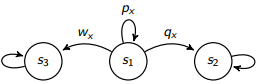
\includegraphics[scale=1.2]{Bilder/Zustandsmodell_Leben1.png}
\end{figure}
\begin{figure}[ht]
	\centering
	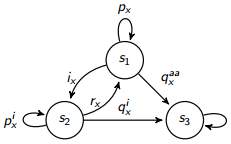
\includegraphics[scale=1.2]{Bilder/Zustandsmodell_Leben2.png}
\end{figure}

\vspace{1cm}
\subsubsection{Sterbetafeln}
Es gibt zwei verschiedene Arten: Periodentafel und Generationstafel. \\
Bei Erlebensfallrisiko mit aufgeschobener Leibrente: Generationentafel. Im Gegensatz zu Periodentafel berücksichtigt die Generationssterbetafel die Sterbewahrscheinlichkeit der jeweiligen Generation des Versicherten -> niedrigere Sterbewahrscheinlichkeit der jüngeren Generation\\
Unterschied DAV 2004 R Tafel und Destatis: DAV für Einschätzung des Erlebensfallrisikos verwendet (Sicherheitsabschläge enthalten). Destatis enthält keine Sicherheitszu- oder abschläge. Außerdem anderes Kollektiv (Versicherte, Gesamtbevölkerung)
Todesfallrisiko: Periodentafel nutzen. Stornowahrscheinlichkeiten sind
erforderlich, wenn bei Storno nicht die Deckungsrückstellung ausbezahlt wird (Cantelli)

In der Lebensversicherung kommen Sterbetafeln der DAV zum Einsatz.\\
Unterscheidung: \\
- 1. Ordnung: Werte enthalten Sicherheiten\\
- 2. Ordnung: Werten entsprechen Erwartungswert

\begin{figure}[ht]
	\centering
	\includegraphics[scale=1]{Bilder/SterbetafelBsp2.png}
\end{figure}
Außerdem stellt die DAV Invaliditätswahrscheinlchkeiten zur Verfügung. Das enthält Wahrscheinlichkeiten zur Sterblichkeit von Invaliden sowie Reaktivierung. Ebenfalls 1. und 2. Ordnung

\subsubsection{Rechnugszins}
Für Rechnungszins der Prämienkalkulation:
\begin{itemize}
\item Einschränkung der Vorsichtsprinzip
\item aber: im Prinzip frei wählbar -> Festlegung Verantwortung von Aktuaren
\end{itemize}
Rechnungszins für Deckungsrückstellungen:
\begin{itemize}
\item Verträge mit Zinsgarantie:
\begin{itemize}
\item Beachten von HHöchstrechnungszins aus §2 (1) DeckRV
\item Rechnungszins bei Vertragabschluss gilt für ganze Laufzeit
\end{itemize}
\item Abweichungen zun Rechnungszins der Prämienkalkulation möglich
\end{itemize}

\subsubsection{Kosten}
\begin{itemize}
\item Abschlusskosten ($\alpha$-Kosten):\\
zu beachten ist Höchstzillmersatz aus §4 (1) DeckRV kosten für Abschlussprovision, Fixkosten im Außendienst, Werbung, Angebotserstellung, Policierung, etc
\item Inkassokosten ($\beta$- Kosten):\\
Kosten für Beitragseinzug, Agenturinkasso, etc.
\item Verwaltungskosten ($\gamma$-Kosten):
Kosten für die Bestandsverwaltung, Bearbeitung von Leistungen, Vertragsänderungen, etc.
\end{itemize}

\subsubsection{Lebensversicherungsprodukte (Auswahl)}
\begin{itemize}
\item Risikoversicherungen: einmalige Zahlung im Todesfall, bspw. Risikolebensversicherung, Todesfallversicherung
\item Kapitalversicherungen: einmalige Zahlung im Erlebensfall, bspw. Erlebensfallversicherung, Gemische Versicherung
\item Rentenversicherung: regelmäßige Zahlungen im Erlebensfall, bspw. sofort beginnende Rentenversicherung, aufgeschobene Rentenversicherung
\end{itemize}

\subsubsection{Wiederholung}
\begin{itemize}
\item Person zum Zeitpunkt $t=0$ mit Alter $x$, dann gilt:
\begin{equation}
\tensor[_{s}]{B}{}_x^L = \sum_{k\geq 0} v^k \cdot \tensor[_k]{p}{}_x \cdot \tensor[_k]{\hat{L}}{}_x
\end{equation}
mit $\tensor[_k]{\hat{L}}{}_x$ Erwartungswert des barwerts aller Leistungen, die mit dem Erreichen des Alters $x+k$ in der HGSH verbunden sind

\item Erlebensfallversicherung: V-Summe $S$ wird bei Erlebens des Zeitpunkts $n$ ausgezahlt: $\tensor[_{s}]{B}{}_x^L = E(L) = v^n \cdot \tensor[_n]{p}{}_x\cdot S = S \cdot \tensor[_n]{E}{}_x$
\item Risikolebensversicherung: V-Summe $S$ wird ausgezahlt bei Tod bis Zeitpunkt $n$: $\tensor[_{s}]{B}{}_x^L = E(L) = \sum_{k=0}^{n-1} v^k \cdot \tensor[_k]{p}{}_x \cdot q_{x+k} \cdot v \cdot S = S \cdot \tensor[_{|n}]{A}{}_x$
\end{itemize}

\subsubsection{Standardformeln und Bezeichnungen}
$x$-jährige Person, Vertrag mit Laufzeit $n$ Jahre, V-Summe $S$ und Zins $i$. Ab Punkt 3: Rentenhöhen betrage $R$ und wird jährlich vorschüssig bezahlt.
\begin{itemize}
\item Gemischte Versicherung: Leistung bei Tod innerhalb der Laufzeit oder bei Erleben Laufzeitende: \\
$E(L) = S\cdot (\tensor[_{|n}]{A}{}_x + \tensor[_n]{E}{}_x) =: S\cdot A_{x:n}$
\textbf{Hier um letztes n eigentlich zwei Linien, aber wie?}
\item Todelfallversicherung: Leistung bei Tod ($\omega$ kalkulatorisches Höchstalter) \\
$E(L) = S \cdot \tensor[_{|\omega -x}]{A}{}_x =: S\cdot A_x$
\item Leibrente:\\
$E(L) = R + R \cdot \tensor[_1]{E}{}_x + r \cdot \tensor[_2]{E}{}_x + ... =: R \cdot \text{\textit{ä}}_x$
\item Aufgeschobene Leibrente um $m$ Jahre:\\
$E(L)= R \cdot \tensor[_m]{E}{}_x + R \cdot \tensor[_{m+1}]{E}{}_x + ... =: R \cdot \tensor[_{m|}]{\text{\textit{ä}}}{}_x$ \\
Erwartungswert des Erfüllungsbetrags: \\
$\tensor[_0]{B}{}_x^L = R \cdot \sum_m v^m \cdot \tensor[_m]{p}{}_x = R \cdot \tensor[_{m|}]{\text{\textit{ä}}}{}_x$
\item Temporäre Leibrente mit Dauer von $n$ Jahre: \\
$E(L) = R + R \cdot \tensor[_1]{E}{}_x + R \cdot \tensor[_2]{E}{}_x + ... + R \cdot \tensor[_{n-1}]{E}{}_x =: R \cdot \text{\textit{ä}}_{x:n} $ \textbf{Hier um letztes n eigentlich zwei Linien, aber wie? Folie 25}
\end{itemize}

\subsubsection{Umgang mit Kosten}
\begin{itemize}
\item Abschlusskosten (blau exemplarisch):\\
- \textcolor{blue}{einmalig} zu Vertragsbeginn: $\alpha^Z$ (Promillesatz) der \textcolor{blue}{Beitragssumme}\\
- \textcolor{blue}{jährlich vorschüssig $\alpha^\gamma$} (Promillesatz) der V-Summe
\item Inkassokosten: \textcolor{blue}{jährlich vorschüssig $\beta$} des jährlichen Beitrags
\item Verwaltungskosten: \textcolor{blue}{jährlich vorschüssig $\gamma$} der V-Summe
\end{itemize}
Leistungsbarwert der Kosten: (\textbf{zwei Striche)}
\begin{equation}
\alpha^Z \cdot n \cdot P + \alpha^\gamma \cdot S \cdot \text{\textit{ä}}_{x:n} + \beta \cdot P \cdot \text{\textit{ä}}_{x:n} + \gamma \cdot S \cdot \text{\textit{ä}}_{x:n}
\end{equation}

\subsubsection{Prämien}
\begin{itemize}
\item Einmalprämie $P$ zu Vertragsbeginn, $P_0=P$ und $P_1=P_2=...=0$: $\tensor[_0]{B}{}_x^P = P$
\item Laufende konstante Prämie $P$ jährlich vorschüssig, $P_0=P_1=...=P_{n-1}=P$, $P_n=0$: $P\cdot ä_{x:n}$ (\textbf{Striche})
\item Laufende konstante Prämie $P$ vorschüssig für $m<n$ Jahre: $P_0=...=P_{m-1}=P$, $P_m=P_{m+1}=P_n=0$: $P\cdot \text{\textit{ä}}_{x:m}$ (\textbf{Striche})
\end{itemize}

\subsubsection{Kosten}
\begin{itemize}
\item $\alpha^Z$: einmalige Abschlusskosten
\item $\alpha^Y$: Abschlusskosten während Vertrag
\item $\beta$: Inkassokosten
\item $\gamma_1$: Verwaltungkosten bis z.B. Renteneintritt
\item $\gamma_2$: Verwaltungkosten während z.B. Rente
\end{itemize}

\subsubsection{Äquivalenzprinzip für einen Vertrag}
\textbf{Striche um ms}
\begin{equation}
P \cdot \text{\textit{ä}}_{x:m} = R \cdot \tensor[_{|m}]{\text{\textit{ä}}}{}_x + \alpha^Z \cdot m \cdot P + ((\alpha^\gamma + \gamma_1)\cdot R + \beta \cdot P) \cdot \text{\textit{ä}}_{x:m} + \gamma_2 \cdot R \cdot \tensor[_{|m}]{\text{\textit{ä}}}{}_x
\end{equation}

\subsubsection{Rekursiver Ansatz Prämienkalkulation}
Betrachten LV-Vertrag mit Laufzeit $n$ Jahre. Prämien können rekursiv bestimmt werden. Ausgangspunkt ist versicherungsmathematische Bilanzgleichung für alle $m\geq 0$ und $\tensor[_n]{V}{}_x=0$ und Dauer Prämienzahlung $a$:
\begin{equation}
\begin{aligned}
\tensor[_m]{V}{}_x & = \tensor[_m]{\hat{L}}{}_x - \tensor[_m]{\hat{P}}{}_x + v \cdot p_{x+m} \cdot \tensor[_{m+1}]{V}{}_x \\
& =S \cdot v \cdot q_{x+m} + v\cdot p_{x+m} \cdot \tensor[_{m+1}]{V}{}_x + \gamma \cdot S + \begin{cases}
	a \cdot \alpha^Z \cdot P + \beta \cdot P - P & \text{für } m=0 \\
	\beta \cdot P + P & \text{für } 0<m< a \\
	0 & \text{für } a\leq m < n
	\end{cases}
\end{aligned}
\end{equation}

Wir erhalten Gleichungen für $\tensor[_{n-1}]{V}{}_x$, $\tensor[_{n-2}]{V}{}_x$ bis $ \tensor[_0]{V}{}_x$ \\
Gesucht ist dann Prämienzahlungsstrom $P$, sodass $\tensor[_0]{V}{}_x - \text{Anfangskapital} =0$ (Bsp in Skript)\\

\large \textbf{Überschussbeteiligung}
\normalsize 
\subsubsection{Rechtliche Grundlagen}

Bei Kalkulation von Beiträgen und Leistungen vorsichtige Herangehensweise, daher idR Überschüsse.
\begin{itemize}
\item Versicherungsvertragsgesetz (§153 (1) VVG)
\begin{itemize}
\item Beteiligung der VN am Überschuss und Bewertungsreserven
\item Ausnahme: Beteiligung ausgeschlossen
\end{itemize}
\item Versicherungsaufsichtsgesetz (§139 (1) VAG)
\begin{itemize}
\item Direkte Zuteilung der Überschüsse oder
\item Zuführung zur Rückstellung für Beitragsrückerstattung (RfB)
\end{itemize}
\end{itemize}
Regelungen, die angemessen Beteiligung der VN am Überschuss sicherstellen (Mindestzuführungsverordnung): Überschüssen werden größtenteils an VN zurückgegeben, Verluste tragen zu großen Teilen die Eigentümer, Asymmetrie im Geschäftsmodell der dt. Lebensversicherung

\begin{figure}[ht]
	\centering
	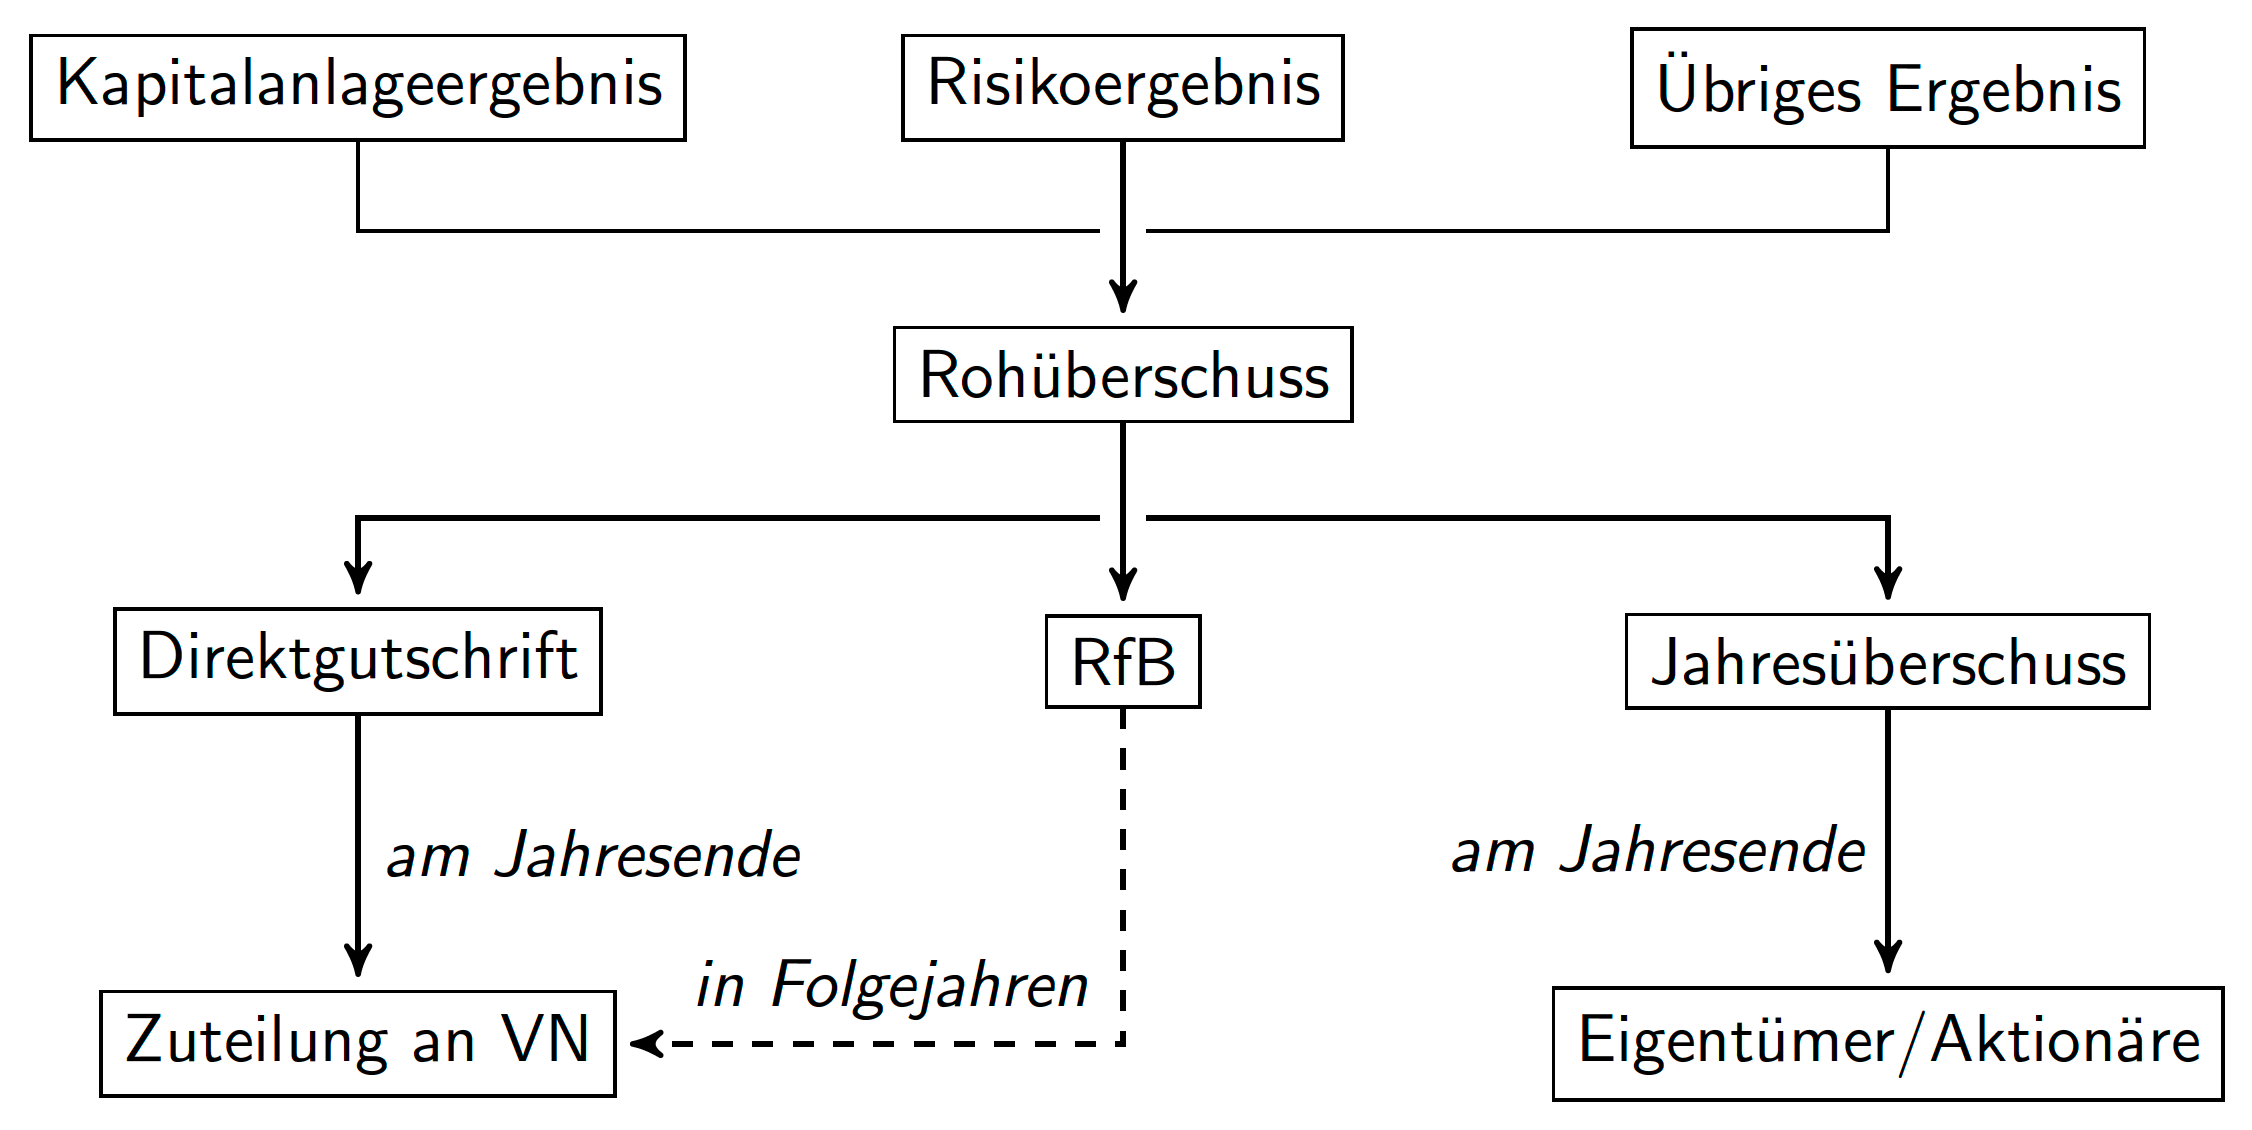
\includegraphics[width= 0.8\textwidth]{Bilder/Ueberschuss.png}
\end{figure}

\subsubsection{Kontributionsgleichung}
Ermitteln von Rohüberschuss kann pro Vertrag mit Kontributionsgleichung \\
Wir betrachten: LV-Vertrag nach $m$ Jahren, Prämienzahlung $P$, Erlebensfallleistung $R$ vorschüssig, Kosten $K$, Todesfallleistung $T$ nachschüssig, tatsächlicher Zins: $\widetilde{i}$, tatsächliche Sterberate $\widetilde{q}$, tatsächliche Kosten $\widetilde{K}$


\begin{figure}[ht]
	\centering
	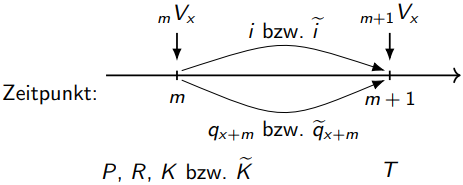
\includegraphics[width = .8\textwidth]{Bilder/Kontributionsgleichung.png}
\end{figure}

Mit kalkulatorischen Größen (Mit tatsächlichen analog): \\
Einnahmen: $E=(\tensor[_m]{V}{}_x + P) \cdot (1+i)$\\
Ausgaben: $A=q_{x+m} \cdot T + (R+K) \cdot (1+i) + (1-q_{x+m})\cdot \tensor[_{m+1}]{V}{}_x$\\
Rohüberschuss im $(m+1)$-ten Jahr:
\begin{align}
=(\tensor[_m]{V}{}_x + P - R - \widetilde{K}) \cdot (\widetilde{i}-i) + (T -\tensor[_{m+1}]{V}{}_x) \cdot (q_{x+m} - \widetilde{q}_{x+m})+(K - \widetilde{K} ) \cdot (1+i) \\ = \text{Zinsergebnis + Risikoergebnis + Kostenergebnis}
\end{align}


\subsubsection{Rückstellung zur Beitragsrückerstattung}
Die Rückstellung für Beitragsrückerstattung (RfB) ist Besonderheit der dt LV:
\begin{itemize}
\item Zeitliche Trennung des Aufwands für Überschussbeteiligung und der zugehörigen Auszahlung: (Vorstand, Aufsichtsrat und Aktuar beschließen Überschussdeklaration)
\item Ziel: Deklaration einer relativ stabilen Überschussbeteiligung
\item Drei Komponenten der RfB: gebundene RfB, Schlussüberschussanteilfonds (SÜA-Fonds), freie RfB
\item Rechtliche Grundlage: Versicherungsaufsichtsgesetz §140 VAG
\item Für überschussberechtigte Verträge gelten folgende Untergrenzen:
\begin{itemize}
\item 90\% der anzurechn. Kapitalerträge (Abzüglich Zinsen)
\item 90\% des Risikoergebnis
\item 50\% des übrigen Ergebnis
\end{itemize}
\item Anmerkungen:
\begin{itemize}
\item Übriges Ergebnis umfasst alle Ergebnisquellen außer Risiko und Kapitalanlage
\item Negative Kapitalanlageergebnisse können verrechnet werden
\item Negatives Risikoergebnis und übriges Ergebnis werden genullt
\end{itemize}
\item Mindestzuführung kann mit Zustimmung der BaFin reduziert werden, um:
\begin{itemize}
\item den Solvabilitätsbedarf für die überschussberechtigten Verträge des Gesamtbestands
\item unvorhersehbare Verluste aus Kapitalanlage-, Risiko- oder übrigen Ergebnis
\item den Erhöhungsbedarf in der Deckungsrückstellung
\end{itemize}
\end{itemize}

\subsubsection{Bewertungsreserven}
Bewertungsreserven (alternativ: Stille Reserven) einer Kapitalanlage (z. B. eines Wertpapiers) entstehen, wenn der Zeitwert dieser Kapitalanlage
über dem Buchwert der Kapitalanlage liegt. Im anderen Fall (Zeitwert kleiner
als Buchwert) entstehen stille Lasten.

\subsubsection{Rechtliche Grundlagen}
Durch Bilanzierung von Kapitalanlagen nach Niederwertprinzip entstehen Bewertungsreserven:
\begin{itemize}
\item Versicherungsvertragsgesetz (§153 (3) VVG)
\begin{itemize}
\item Bewertungsreserven jährlich neu ermitteln
\item nach verursachungsorientiertem Verfahren zuordnen
\item mind. hälftige Zuteilung bei Vertragsende bzw bei Renten: nach Ansparphase
\end{itemize}
\item Versicherungsaufsichtsgesetz: best festverzinslichen Anlagen und Zinsabsicherungsgeschäften: Nur Teil über Sicherungsbedarf relevant
\end{itemize}
Beteiligung an Bewertungsreserven:
\begin{itemize}
\item Erweiterung der klassischen Zinsgewinnbeteiligung an noch nicht realisierten Erträgen (aber: Einbeziehung der stillen lasten unzulässig)
\item Unterscheidung der Bewertungsreserven: aus festverzinslichen Kapitalanlagen und andere Kapitalanlagen (z.B. Aktien, Immobilien)
\end{itemize}

\subsubsection{Sicherungsbedarf}
Beteiligung an den Bewertungsreserven aus festverzinslichen Wertpapieren nur, wenn Sicherungsbedarf überschritten\\
Berechnung Sicherungsbedarf: Differenz aus Deckungsrückstellung mit "Bezugszins" und Deckungsrückstellung mit Rechnungszins

\subsubsection{Anspruchberechtigung}
Beteiligung an den Bewertungsreserven nur für anspruchsberechtigte Vertäge
\begin{itemize}
\item anspruchberechtigt: Kapitalbildende klassische Lebens- und Rentenversicherungen
\item nicht anspruchberechtigt: Fondsgebundene Versicherungen und Versicherungen mit Deckungsrückstellungen, die lediglich zur Glättung der Risikoverlaufs bei konstanten Prämien dienen
\end{itemize}

\chapter{Krankenversicherung}

\subsubsection{Allgemeines}
\begin{itemize}
	\item duales System (PKV, GKV)
	\item versicherungsfreie Personen: Gehalt oberhalb der Grenze, beihilfeberechtigte Personen, Personen mit freier Heilfürsorge
	\item VVG: Krankheitskostenversicherung für ambulante und stationäre Behandlung, max. 5000€ Selbstbehalt
	\item Unterscheidung substituive (ersetzt ganz oder teilweise den Schutz des gesetzlichen Systems, muss nach Art der Lebensversicherung betrieben) und nicht substituive Krankenversicherung (kann nach Art der Lebensversicherung betrieben werden)
	\item Wechsel in der PKV: 
		\begin{itemize}
		\item keine Übertragung der Altersrückstellung für nicht-substituive KV, subst. KV mit Beginn vor 01.01.2009 und Krankentagegeldversicherung
		\item Übertragung für subst. KV mit Beginn nach 01.01.2009 (Wert: gleicher, der sich bei Basistarif ergeben hätte)
		\end{itemize}
	\item Periodensterbetafel: zu einem bestimmten Zeitraum
	\item Generationensterbetafel: zu einer Geburtskohorte
	\item Sterbetafel mit Referenzjahr: Prognose
\end{itemize}

\subsubsection{Zustandsmodell KV - Teil 1}
\begin{figure}[ht]
	\centering
	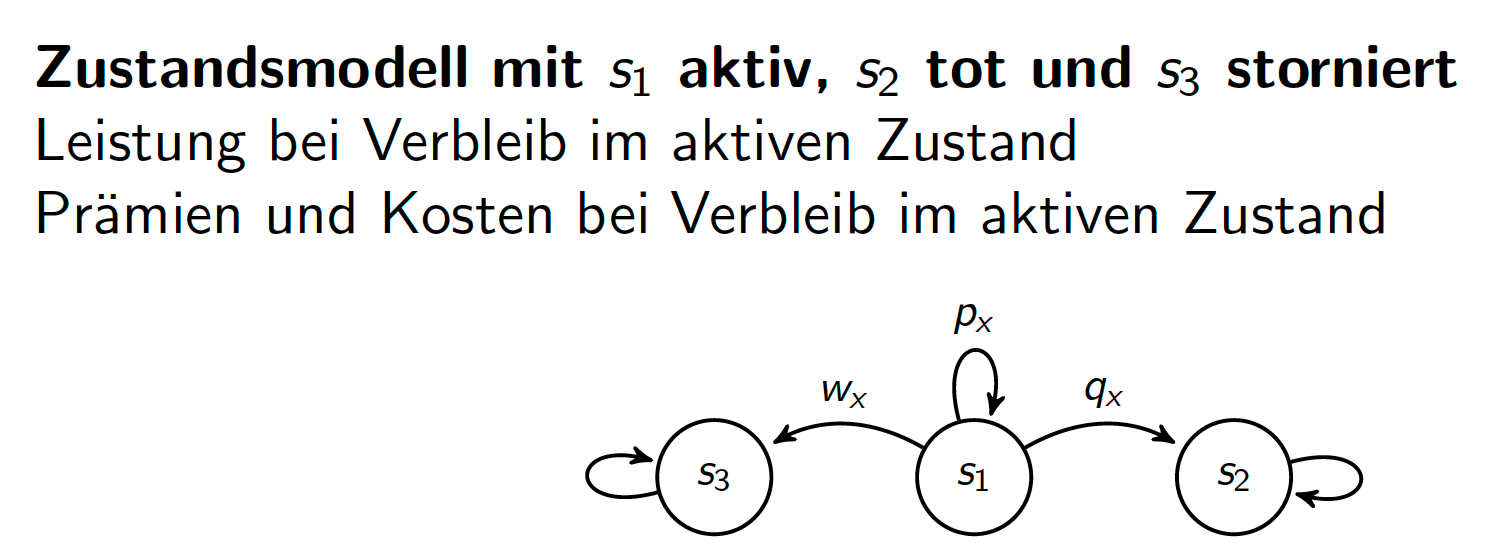
\includegraphics[width = .8\textwidth]{Bilder/ZustandModellKV.png}
\end{figure}

\subsubsection{Rechnungsgrundlagen PKV}
\begin{itemize}
	\item Rechnungszins: Obergrenze 3,5$\%$, orientiert sich an AUZ, nicht notwendigerweise für ganze Laufzeit garantiert
	\item Ausschreideordnung: bei Tod und Storno. Für $x$-jährige Person $q^{Tod}_x \eqqcolon q_x$, $q_x^{Storno} \eqqcolon w_x$, Verbleibewahrscheinlichkeit $p_x=1-q_x-w_x$
	\item Übertrittswahrscheinlichkeiten
	\item Sonstige Zuschläge
	\item Praxis: 
		\begin{itemize}
			\item Doku jedes Tarifs in technischen Berechnungsgrundlagen
			\item Rechnungszins orientiert sich am AUZ (Aktuarieller Unternehmenszins)
			\item Ausscheideordnung: üblicherweise Verbandswerte wegen zu kleiner Bestände, unternehmenseigene Werte zulässig
		\end{itemize}
\end{itemize}

\subsubsection{Sterbewahrscheinlichkeit Herleitung}
\begin{itemize}
	\item[$\rightarrow$] Praxis: jährlich neue Sterbetafel veröffentlicht
	\item[1.] Schätzung der rohen Sterbewahrscheinlichkeiten
	\item[2.] Ausgleich der rohen Sterbewahrscheinlichkeiten
	\item[3.] Berücksichtigung Sicherheitsabschlag
	\item[4.] Bestimmung Trend, Projektion um 7 Jahre
	\item[5.] Abgleich mit Vorjahreswerten 
\end{itemize}

\subsubsection{Kopfschäden}
\begin{itemize}
	\item erwartete Leistung für eine Person
	\item Beobachtungszeitraum: 12 Monate
	\item abhängig von Tarif und Alter
	\item Notation für $x$-jährige Person: $K_x$
	\item Besonderheiten:
		\begin{itemize}
			\item Wartezeit- und Selektionsersparnisse: Neukunden sind bessere Risiken als gleichaltrige Kunden (Ursachen: gewisse Leistungen erst nach 3 Monaten, Risikoprüfung bei Vertragsabschluss)
			\item S-Kosten: Leistungsausgaben bedingt durch Schwangerschaft, Geburt und Mutterschutz (Umlage durch allg. Gleichbehandlungsgesetz, geschlechtsunabh. Kalkulation)
			\item Tatsächlicher Grundkopfschaden: abzüglich Nettorisikozuschläge, einschlie{\ss}lich Leistungen wegen Schwanger- und Mutterschaft, rechnungsmä{\ss}ige Profilwerte nutzen, für jedes Alter abzugrenzen
		\end{itemize}
\end{itemize}

\subsubsection{Rusam-Methode}
\begin{itemize}
	\item fixiere Alter $x_0$, bestimme für jedes Alter $k_x \coloneqq \frac{K_x}{K_{x_0}}$
	\item $k_x$: normierter Kopfschaden zum Alter $x$
	\item Gesamtheit aller $k_x$ hei{\ss}t Profil
	\item Grundkopfschaden: $G \coloneqq K_{x_0} \Rightarrow K_x=k_x \cdot G$
	\item Zerlegung in Grundkopfschaden und Profil ist Standard bei Bestimmung der Kopfschäden in der PKV
	\item Vorteile: Profile für mehrere Tarife nutzbar und im Zeitablauf stabil, vereinfachen Kalkulation
\end{itemize}

\subsubsection{Kosten und Zuschläge}
\begin{itemize}
	\item Sicherheitszuschlag verpflichtend, mind. 5$\%$ der Bruttoprämie, nicht in anderen Rechnungsgrundlagen enthalten
	\item ansetzbare Kosten: Abschlusskosten, Verwaltungskosten, KV-spezifische Zuschläge
	\item Bei Festlegung zu beachten: Einschränkungen der Höhe bei unmittelbaren Abschlusskosten, nur altersunabhängige absolute Kostenzuschläge erlaubt
\end{itemize}

\subsubsection{Überprüfung Rechnungsgrundlagen}
\begin{itemize}
	\item Voraussetzung für Prämienanpassung: „... nicht nur als vorübergehend anzusehenden Veränderung einer für die Prämienkalkulation ma{\ss}geblichen Rechnungsgrundlage ...“
	\item ma{\ss}gebliche Rechnungsgrundlagen: Versicherungsleistung (Kopfschaden) und Sterbewahrscheinlichkeiten
\end{itemize}

\subsubsection{Auslösender Faktor für Schäden}
\begin{itemize}
	\item Überprüfung der Rechnungsgrundlage der Kopfschäden durch Vergleich erforderlicher und kalkulatorischer Leistungen mindestens jährlich
	\item Auslösender Faktor für Versicherungsleistungen (Kopfschäden): $AF_{Schaden} \coloneqq \frac{S^{erf}}{S^{kalk}}$
	\item Prämien überprüfen, falls $|1-AF_{Schaden}|>10\%$ und Änderung nicht nur vorübergehend
	\item Bestimmung der erforderlichen Leistungen auf Basis einer Extrapolation der letzten drei Jahre
	\item Tatsächlicher Grundkopfschaden in einem Jahr ($S$ abgegrenzter Schaden, $n_x$ abgegrenzter mittlerer Bestand, $k_x$ rechn.mä{\ss}iges Profil für Alter $x$:
		\begin{equation}
			G= \frac{S}{\sum_x n_x \cdot k_x}
		\end{equation}
	\item Extrapolierter Grundkopfschaden um 18 Monate unter Verwendung von $G_t, G_{t-1}, G_{t-2}$:
	\begin{equation}
		G^{(ext)}=\frac{3}{2} \cdot (G_t - G_{t-2})+\frac{1}{3} \cdot(G_{t-2}+G_{t-1}+G_t)
	\end{equation}
	\item erforderliche Versicherungsleistungen:
		\begin{equation}
			S^{erf} \coloneqq \sum_x n_x \cdot G^{(ext)} \cdot k_x^{rech}
		\end{equation}
	\item kalkulatorische Versicherungsleistungen:
		\begin{equation}
			S^{kalk} \coloneqq \sum_x n_x \cdot G^{(rech)} \cdot k_x^{rech}
		\end{equation}
	\item mit: $n_x$ abgegrenzte mittlere Bestandsgrö{\ss}e im Alter $x$ und $G^{(ext)}$ extrapolierter Grundkopfschaden
	\item Ergebnis: Vergleich der Grundkopfschäden
\end{itemize}

\subsubsection{Auslösender Faktor für Sterblichkeit}
\begin{itemize}
	\item mindestens jährlicher Vergleich von erforderlichen und kalkulatorischen Sterbewahrscheinlichkeiten (Leistungsbarwerte vergleichen)
	\item auslösender Faktor Sterblichkeit:
		\begin{equation}
			AF_{Sterb} \coloneqq max\biggl\{\frac{1}{25} \cdot \sum_{x=21}^{45} \frac{A_x^{(erf)}}{A_x^{(kalk)}}, \frac{1}{25} \cdot \sum_{x=46}^{70} \frac{A_x^{(erf)}}{A_x^{(kalk)}}, \frac{1}{25} \cdot \sum_{x=71}^{95} \frac{A_x^{(erf)}}{A_x^{(kalk)}}\biggr\}
		\end{equation}
	\item Überprüfung der Prämien, wenn $|1-AF_{Sterb}|>5\%$
	\item Bestimmung des Leistungsbarwerts ohne Storno-Whk.
	\item bei Krankengeld: Betrachtung Alter 21-45 und 46-65
	\item Leistungsbarwert mit kalkulatorischen Sterbewahrscheinlichkeiten:
		\begin{equation}
			A_x^{(kalk)}=\sum_{t\geq 0} v^t \cdot \tensor[_t]{p}{}_x \cdot K_{x+t}
		\end{equation}
	\item Leistungsbarwert mit erforderlichen Sterbewahrscheinlichkeiten
		\begin{equation}
			A_x^{(erf)}=\sum_{t\geq 0} v^t \cdot \tensor[_t]{p}{}_x^{BaFin} \cdot K_{x+t}
		\end{equation}
	\item $q_x^{(BaFin)}$ Sterblichkeit aus aktueller PKV-Sterbetafel
\end{itemize}

\subsubsection{Zustandsmodell KV - Teil 2}
\begin{itemize}
	\item nach $t$-jährigem Verbleib in Hauptgesamtheit: 
		\begin{equation}
			\tensor[_t]{\hat{L}}{}_x = K_{x+t}+w_{x+t} \cdot v \cdot \text{\textit{Ü}}_{x+t+1}
		\end{equation}
	\item $\text{\textit{Ü}}_{x+t+1}$ ist die Übertragungswertzahlung bei Storno in Vertragsjahr $t+1$, Rechnung mit $\text{\textit{Ü}}_{x}=0$
	\item Leistungsbarwert \textcolor{red}{mit Übertragungswertzahlung (ab 2009)}:
		\begin{align}
			A_x \coloneqq \sum_{t=0}^{\omega-x} v^t \cdot \tensor[_t]{p}{}_x \cdot (K_{x+t} \color{red} + w_{x+t}\cdot v \cdot \text{\textit{Ü}}_{x+t+1} \color{black})
		\end{align}
\end{itemize}

\subsubsection{Prämienanpassung}
\begin{equation}
	\tensor[_{m}]{V}{}_x + B_u^{a/n} \cdot \text{\textit{ä}}_u = A_u + \Delta \cdot B_u^{a/n} \cdot \text{\textit{ä}}_u + \gamma \cdot \text{\textit{ä}}_u + \alpha _u^{''} \cdot max \{B_u^{a/n}-B^a;0\}
\end{equation}

\subsubsection{Altenproblem}
	\begin{equation}
		P_u^{a/n}=(1+\lambda) \cdot P^a + \lambda \cdot (P_u^a-P^a)
	\end{equation}

\subsubsection{Äquivalenzgleichung}
\begin{itemize}
	\item verallgemeinertes Äquivalenzprinzip (Abschlussalter $x$, jetzt $x+m$)
		\begin{equation}
			\tensor[_m]{V}{}_x + B^a \cdot \text{\textit{ä}}^{\ a}_u = A_u^a + \Delta^a \cdot B^a \cdot \text{\textit{ä}}^{\ a}_u + \gamma^a \cdot \text{\textit{ä}}^{\ a}_u
		\end{equation}
	\item d.h. Altersrückstellungen zzgl. erw. Barwert aller zukünftiger Prämien finanziert Leistungsbarwert der Versicherungsleistungen und Kosten
	\item ohne Kosten: 
		\begin{equation}
			\tensor[_m]{V}{}_x^{(netto)} + P^a \cdot \text{\textit{ä}}^{\ a}_u = A_u^a
		\end{equation}
\end{itemize}






\end{document}